% Options for packages loaded elsewhere
\PassOptionsToPackage{unicode}{hyperref}
\PassOptionsToPackage{hyphens}{url}
\documentclass[
  11pt,
]{article}
\usepackage{xcolor}
\usepackage[margin=1in]{geometry}
\usepackage{amsmath,amssymb}
\setcounter{secnumdepth}{5}
\usepackage{iftex}
\ifPDFTeX
  \usepackage[T1]{fontenc}
  \usepackage[utf8]{inputenc}
  \usepackage{textcomp} % provide euro and other symbols
\else % if luatex or xetex
  \usepackage{unicode-math} % this also loads fontspec
  \defaultfontfeatures{Scale=MatchLowercase}
  \defaultfontfeatures[\rmfamily]{Ligatures=TeX,Scale=1}
\fi
\usepackage{lmodern}
\ifPDFTeX\else
  % xetex/luatex font selection
\fi
% Use upquote if available, for straight quotes in verbatim environments
\IfFileExists{upquote.sty}{\usepackage{upquote}}{}
\IfFileExists{microtype.sty}{% use microtype if available
  \usepackage[]{microtype}
  \UseMicrotypeSet[protrusion]{basicmath} % disable protrusion for tt fonts
}{}
\makeatletter
\@ifundefined{KOMAClassName}{% if non-KOMA class
  \IfFileExists{parskip.sty}{%
    \usepackage{parskip}
  }{% else
    \setlength{\parindent}{0pt}
    \setlength{\parskip}{6pt plus 2pt minus 1pt}}
}{% if KOMA class
  \KOMAoptions{parskip=half}}
\makeatother
\usepackage{color}
\usepackage{fancyvrb}
\newcommand{\VerbBar}{|}
\newcommand{\VERB}{\Verb[commandchars=\\\{\}]}
\DefineVerbatimEnvironment{Highlighting}{Verbatim}{commandchars=\\\{\}}
% Add ',fontsize=\small' for more characters per line
\usepackage{framed}
\definecolor{shadecolor}{RGB}{248,248,248}
\newenvironment{Shaded}{\begin{snugshade}}{\end{snugshade}}
\newcommand{\AlertTok}[1]{\textcolor[rgb]{0.94,0.16,0.16}{#1}}
\newcommand{\AnnotationTok}[1]{\textcolor[rgb]{0.56,0.35,0.01}{\textbf{\textit{#1}}}}
\newcommand{\AttributeTok}[1]{\textcolor[rgb]{0.13,0.29,0.53}{#1}}
\newcommand{\BaseNTok}[1]{\textcolor[rgb]{0.00,0.00,0.81}{#1}}
\newcommand{\BuiltInTok}[1]{#1}
\newcommand{\CharTok}[1]{\textcolor[rgb]{0.31,0.60,0.02}{#1}}
\newcommand{\CommentTok}[1]{\textcolor[rgb]{0.56,0.35,0.01}{\textit{#1}}}
\newcommand{\CommentVarTok}[1]{\textcolor[rgb]{0.56,0.35,0.01}{\textbf{\textit{#1}}}}
\newcommand{\ConstantTok}[1]{\textcolor[rgb]{0.56,0.35,0.01}{#1}}
\newcommand{\ControlFlowTok}[1]{\textcolor[rgb]{0.13,0.29,0.53}{\textbf{#1}}}
\newcommand{\DataTypeTok}[1]{\textcolor[rgb]{0.13,0.29,0.53}{#1}}
\newcommand{\DecValTok}[1]{\textcolor[rgb]{0.00,0.00,0.81}{#1}}
\newcommand{\DocumentationTok}[1]{\textcolor[rgb]{0.56,0.35,0.01}{\textbf{\textit{#1}}}}
\newcommand{\ErrorTok}[1]{\textcolor[rgb]{0.64,0.00,0.00}{\textbf{#1}}}
\newcommand{\ExtensionTok}[1]{#1}
\newcommand{\FloatTok}[1]{\textcolor[rgb]{0.00,0.00,0.81}{#1}}
\newcommand{\FunctionTok}[1]{\textcolor[rgb]{0.13,0.29,0.53}{\textbf{#1}}}
\newcommand{\ImportTok}[1]{#1}
\newcommand{\InformationTok}[1]{\textcolor[rgb]{0.56,0.35,0.01}{\textbf{\textit{#1}}}}
\newcommand{\KeywordTok}[1]{\textcolor[rgb]{0.13,0.29,0.53}{\textbf{#1}}}
\newcommand{\NormalTok}[1]{#1}
\newcommand{\OperatorTok}[1]{\textcolor[rgb]{0.81,0.36,0.00}{\textbf{#1}}}
\newcommand{\OtherTok}[1]{\textcolor[rgb]{0.56,0.35,0.01}{#1}}
\newcommand{\PreprocessorTok}[1]{\textcolor[rgb]{0.56,0.35,0.01}{\textit{#1}}}
\newcommand{\RegionMarkerTok}[1]{#1}
\newcommand{\SpecialCharTok}[1]{\textcolor[rgb]{0.81,0.36,0.00}{\textbf{#1}}}
\newcommand{\SpecialStringTok}[1]{\textcolor[rgb]{0.31,0.60,0.02}{#1}}
\newcommand{\StringTok}[1]{\textcolor[rgb]{0.31,0.60,0.02}{#1}}
\newcommand{\VariableTok}[1]{\textcolor[rgb]{0.00,0.00,0.00}{#1}}
\newcommand{\VerbatimStringTok}[1]{\textcolor[rgb]{0.31,0.60,0.02}{#1}}
\newcommand{\WarningTok}[1]{\textcolor[rgb]{0.56,0.35,0.01}{\textbf{\textit{#1}}}}
\usepackage{longtable,booktabs,array}
\usepackage{calc} % for calculating minipage widths
% Correct order of tables after \paragraph or \subparagraph
\usepackage{etoolbox}
\makeatletter
\patchcmd\longtable{\par}{\if@noskipsec\mbox{}\fi\par}{}{}
\makeatother
% Allow footnotes in longtable head/foot
\IfFileExists{footnotehyper.sty}{\usepackage{footnotehyper}}{\usepackage{footnote}}
\makesavenoteenv{longtable}
\usepackage{graphicx}
\makeatletter
\newsavebox\pandoc@box
\newcommand*\pandocbounded[1]{% scales image to fit in text height/width
  \sbox\pandoc@box{#1}%
  \Gscale@div\@tempa{\textheight}{\dimexpr\ht\pandoc@box+\dp\pandoc@box\relax}%
  \Gscale@div\@tempb{\linewidth}{\wd\pandoc@box}%
  \ifdim\@tempb\p@<\@tempa\p@\let\@tempa\@tempb\fi% select the smaller of both
  \ifdim\@tempa\p@<\p@\scalebox{\@tempa}{\usebox\pandoc@box}%
  \else\usebox{\pandoc@box}%
  \fi%
}
% Set default figure placement to htbp
\def\fps@figure{htbp}
\makeatother
\setlength{\emergencystretch}{3em} % prevent overfull lines
\providecommand{\tightlist}{%
  \setlength{\itemsep}{0pt}\setlength{\parskip}{0pt}}
\usepackage{bookmark}
\IfFileExists{xurl.sty}{\usepackage{xurl}}{} % add URL line breaks if available
\urlstyle{same}
\hypersetup{
  pdftitle={From Oven to Online: A Data-Led, AI-Augmented Go-to-Market Plan for Tyne Artisan Bakery},
  pdfauthor={Student Number: {[}insert{]}},
  hidelinks,
  pdfcreator={LaTeX via pandoc}}

\title{From Oven to Online: A Data-Led, AI-Augmented Go-to-Market Plan
for Tyne Artisan Bakery}
\usepackage{etoolbox}
\makeatletter
\providecommand{\subtitle}[1]{% add subtitle to \maketitle
  \apptocmd{\@title}{\par {\large #1 \par}}{}{}
}
\makeatother
\subtitle{Anchored on Monthly Active Local Customers (MALC) as the North
Star metric}
\author{Student Number: {[}insert{]}}
\date{May 2026}

\begin{document}
\maketitle

{
\setcounter{tocdepth}{3}
\tableofcontents
}
\newpage

\section{Executive Summary}\label{executive-summary}

\begin{quote}
\emph{``Growth is not only about acquiring more customers; it is about
repeatedly creating measurable value for the right customers.''}
\end{quote}

Tyne Artisan Bakery (TAB) is a Newcastle-based artisan bakery with a
strong in-store reputation, but with limited digital presence. This
report develops a data-led and AI-augmented go-to-market plan for the
next \textbf{12--18 months}, anchored around one clear North Star
metric: \textbf{Monthly Active Local Customers (MALC)}. MALC is used
because it connects digital growth directly with repeat local customer
engagement, rather than treating online sales as a one-off acquisition
exercise.

The analysis is based on TAB's two-year transactional dataset covering
\textbf{5,942 orders}, \textbf{4,179 unique customers}, and
\textbf{£120,835 in total revenue} between \textbf{March 2024 and
February 2026}. The findings suggest that TAB should not immediately
pursue broad national e-commerce expansion. Instead, it should first
build a focused, mobile-first, locally targeted online channel for the
North East market, supported by owned media, customer retention, and
selective automation.

\begin{longtable}[]{@{}
  >{\raggedright\arraybackslash}p{(\linewidth - 4\tabcolsep) * \real{0.2148}}
  >{\raggedright\arraybackslash}p{(\linewidth - 4\tabcolsep) * \real{0.2815}}
  >{\raggedright\arraybackslash}p{(\linewidth - 4\tabcolsep) * \real{0.5037}}@{}}
\caption{Table 1: Executive summary of TAB's commercial
baseline}\tabularnewline
\toprule\noalign{}
\begin{minipage}[b]{\linewidth}\raggedright
Metric
\end{minipage} & \begin{minipage}[b]{\linewidth}\raggedright
Value
\end{minipage} & \begin{minipage}[b]{\linewidth}\raggedright
Strategic meaning
\end{minipage} \\
\midrule\noalign{}
\endfirsthead
\toprule\noalign{}
\begin{minipage}[b]{\linewidth}\raggedright
Metric
\end{minipage} & \begin{minipage}[b]{\linewidth}\raggedright
Value
\end{minipage} & \begin{minipage}[b]{\linewidth}\raggedright
Strategic meaning
\end{minipage} \\
\midrule\noalign{}
\endhead
\bottomrule\noalign{}
\endlastfoot
Orders analysed & 5,942 & Sufficient order base for customer, channel
and conversion analysis \\
Unique customers & 4,179 & Shows a sizeable customer pool for
retention-led growth \\
Total revenue & £120,835 & Confirms commercial potential, but not yet a
mature digital engine \\
Average order value & £20.34 & Requires careful acquisition-cost control
before scaling paid media \\
North Star metric & Monthly Active Local Customers (MALC) & Connects
digital growth with repeat local customer engagement \\
Recommended planning horizon & 12--18 months & Allows phased MVP launch,
testing, optimisation and scale-up \\
\end{longtable}

Four core findings shape the recommended plan.

First, \textbf{paid media is not yet economically efficient enough to be
scaled aggressively}. Among paid channels, only Google Search generates
a return above the breakeven threshold, with a ROAS of \textbf{1.14×}.
Meta, TikTok and Other channels remain below breakeven, with ROAS values
of \textbf{0.82×}, \textbf{0.90×} and \textbf{0.62×} respectively. Since
blended customer acquisition cost is estimated at \textbf{£36--£52},
which is well above the average order value of \textbf{£20.34}, TAB
should prioritise organic search, email, referral, local partnerships
and owned social content before increasing paid advertising spend. This
follows the digital marketing argument that acquisition channels should
be judged through customer economics, not traffic volume alone
(Reichheld \& Schefter, 2000; Kannan \& Li, 2017).

\begin{center}
\includegraphics[width=0.95\linewidth]{ISO8005_TAB_Report_files/figure-latex/executive-roas-chart-1} \end{center}

Second, \textbf{the North East should be TAB's launch market for digital
growth}. The North East already contributes \textbf{20.1\% of total
revenue}, making it TAB's strongest and most natural commercial
catchment. Other UK regions show long-tail demand, but they appear more
suitable for later-stage testing rather than immediate expansion.
Therefore, the initial e-commerce proposition should be positioned
around local convenience, artisan quality, gifting, subscriptions and
community identity.

Third, \textbf{the A/B test provides strong evidence for immediate
conversion improvement}. Variant B, the treatment hero banner, achieves
a conversion rate of \textbf{3.65\%}, compared with \textbf{2.86\%} for
the control. This represents a \textbf{27.5\% relative uplift}, with a
statistically significant result of \textbf{z = 6.90, p \textless{}
0.001}. The result meets both practical and statistical thresholds for
rollout. This supports an evidence-based approach to digital product
design, where small interface changes are tested before wider
implementation (Kohavi, Tang \& Xu, 2020).

\begin{center}
\includegraphics[width=0.95\linewidth]{ISO8005_TAB_Report_files/figure-latex/executive-ab-chart-1} \end{center}

Fourth, \textbf{TAB's online platform must be mobile-first and
subscription-led}. Mobile already accounts for approximately
\textbf{69\% of orders}, which means the customer journey must be
designed primarily for smaller screens, faster checkout and low-friction
repeat ordering. Subscription orders represent \textbf{17.7\% of order
volume}, while average monthly churn remains at a manageable
\textbf{4.5\%}. This indicates that subscription-led retention can
provide a more stable revenue base than one-off acquisition. Over time,
AI-supported product recommendations, automated retention messages and
simple demand forecasting can strengthen this repeat-purchase loop
(Taylor \& Letham, 2018).

\begin{center}
\includegraphics[width=0.95\linewidth]{ISO8005_TAB_Report_files/figure-latex/executive-strategy-flow-1} \end{center}

Based on these findings, the recommended solution is a \textbf{Shopify
Basic e-commerce MVP} supported by a thin AI layer. This should include:
\textbf{(i)} LLM-assisted product recommendations, \textbf{(ii)} demand
forecasting using Prophet, and \textbf{(iii)} a GenAI content studio for
menu descriptions, campaign copy and accessible image alt text.

At an indicative 12-month investment of approximately \textbf{£11,500},
the Base scenario assumes \textbf{4\% monthly compound MALC growth}.
Under this scenario, MALC increases from \textbf{430 in February 2026}
to approximately \textbf{690 by February 2027}. If current ordering
frequency and average order value remain broadly stable, monthly revenue
may rise proportionally to approximately \textbf{£18.4k}. In the High
scenario, stronger conversion, retention and subscription adoption could
add approximately \textbf{30\% further upside} by the end of the first
year.

\begin{center}
\includegraphics[width=0.95\linewidth]{ISO8005_TAB_Report_files/figure-latex/executive-malc-scenario-1} \end{center}

Overall, the report recommends that TAB should launch a focused local
e-commerce MVP before pursuing wider national growth. The immediate
objective is not to maximise digital reach, but to build a repeatable
local growth engine. If TAB improves conversion, protects acquisition
economics and increases repeat purchasing, MALC can become a practical
and measurable bridge between artisan brand strength and scalable
digital revenue.

\newpage

\section{Introduction}\label{introduction}

\subsection{Business Context and Problem
Framing}\label{business-context-and-problem-framing}

TAB is a microenterprise: founder-led, fewer than ten staff, and bounded
by the physical reach of its in-store counter and weekend market stall.
The owners want to launch e-commerce (local delivery and
click-and-collect) and build a coherent social presence from scratch,
with modest budgets and limited technical expertise (Assignment Brief,
2026).

The deeper strategic problem is not \emph{the absence of a website}. It
is the \textbf{absence of a measurable digital customer-acquisition and
-retention system}. Without instrumented funnels and a single agreed
metric, every marketing investment becomes a bet rather than an
experiment. This report addresses that gap by sequencing:

\begin{quote}
\begin{enumerate}
\def\labelenumi{(\roman{enumi})}
\tightlist
\item
  \textbf{the metric} that should govern decisions (the North Star);
\item
  \textbf{the MVP} that produces the data; and
\item
  \textbf{the analytics and forecasting} that turn data into
  reallocation.
\end{enumerate}
\end{quote}

\subsection{Methodology}\label{methodology}

\subsubsection{2.1 Overview: The Four-Stage Analytics
Workflow}\label{overview-the-four-stage-analytics-workflow}

This report follows a structured four-stage data-analytics workflow
consistent with the CRISP-DM reference model (Wirth \& Hipp, 2000) and
reinforced by reproducible research practices (Wickham \& Bryan, 2023).
The entire analysis is automated in R and can be re-run from raw data to
final PDF in a single command (\texttt{source("scripts/RUN\_ALL.R")}),
ensuring transparency and auditability.

\begin{figure}

{\centering 
\includegraphics[width=0.95\linewidth]{ISO8005_TAB_Report_files/figure-latex/methodology-overview-flowchart-1} 

}

\caption{Figure 2: End-to-end data analytics workflow from raw Excel to decision-ready insights.}\label{fig:methodology-overview-flowchart}
\end{figure}

\subsubsection{2.2 Stage 1: Data Understanding \&
Preparation}\label{stage-1-data-understanding-preparation}

\textbf{Inputs}: Raw Excel workbook
(\texttt{ISO8005\_TAB\_issued\_AY2526.xlsx}) with 7 sheets: -
\texttt{monthly\_marketing} (24 rows, 27 columns: traffic, CVR, revenue,
ad spend by channel, email, social) - \texttt{paid\_campaigns} (96 rows:
channel, spend, impressions, clicks, conversions, attributed revenue) -
\texttt{web\_analytics} (24 rows: sessions, bounce rate, device/channel
breakdown) - \texttt{orders} (5,942 rows: order date, customer ID,
region, product category, revenue, subscription flag, device) -
\texttt{ab\_test} (122 rows: variant, views, conversions, date) -
\texttt{social\_metrics} (72 rows: platform, followers, posts,
engagements, clicks to site) - \texttt{Data\ Dictionary} (metadata and
formula notes)

\textbf{Process} (Script 01): 1. Load all sheets using
\texttt{readxl::read\_excel()} and apply
\texttt{janitor::clean\_names()} for consistent column naming. 2.
\textbf{Profile each sheet}: Check row counts, column types, missing
values and date ranges. 3. \textbf{Type harmonisation}: Coerce date
columns to \texttt{Date} class; ensure numeric columns are numeric. 4.
\textbf{Quality checks}: Identify null counts, outlier orders (e.g., £0
revenue, future dates), duplicate customer IDs within single orders. 5.
\textbf{Export}: Save cleaned RData objects for downstream scripts.

\textbf{Quality gates}: - No orders with
\texttt{order\_date\ \textgreater{}\ Sys.Date()} - All
\texttt{revenue\ \textgreater{}=\ 0} - \texttt{customer\_id} and
\texttt{order\_id} are non-null for all orders - Date ranges are
consistent (Mar 2024 -- Feb 2026 for monthly tables; longer tails in
transaction tables are investigated)

\textbf{Output}: \texttt{cleaned\_data.RData} (7 cleaned objects);
console profile report.

\subsubsection{2.3 Stage 2: Metric Modelling \& KPI
Computation}\label{stage-2-metric-modelling-kpi-computation}

\textbf{Inputs}: Cleaned data objects from Stage 1.

\textbf{Process} (Script 02):

\begin{verbatim}
## 
##                          CLEANED DATA
##                               |
##                  |-------|-------|-------|-------|
##                  |       |       |       |       |
##             ORDERS   MARKETING  WEB   PAID    AB_TEST
##               SHEET    SHEET   SHEET  SHEET    SHEET
##               (5.9k)   (24mo)  (24mo) (96)     (122)
##                  |       |       |       |       |
##                  v       v       v       v       v
##           ┌─────────────────────────────────┐
##           │   AGGREGATION & CALCULATION     │
##           │   ─────────────────────────────  │
##           │  • CVR = orders / sessions      │
##           │  • AOV = revenue / orders       │
##           │  • CTR = clicks / impressions   │
##           │  • CAC = spend / conversions    │
##           │  • ROAS = revenue / spend       │
##           │  • MALC = distinct customers    │
##           │  • Churn, seasonality, region   │
##           └─────────────────────────────────┘
##                          |
##             |-------|-------|-------|
##             |       |       |       |
##           MONTHLY  PAID    REGION  CHURN &
##          METRICS  PERF    ANALYSIS RETENTION
##           (24 mo)  (by    (by      (trends)
##                   channel) region)
##                  |
##                  v
##          15+ COMPUTED KPIs
##          ─────────────────
##          monthly_metrics, paid_perf,
##          region_mix, seasonality,
##          ab_summary, malc_trend,
##          subscription_summary
\end{verbatim}

\textbf{Key formulas:}

\begin{longtable}[]{@{}
  >{\raggedright\arraybackslash}p{(\linewidth - 6\tabcolsep) * \real{0.1136}}
  >{\raggedright\arraybackslash}p{(\linewidth - 6\tabcolsep) * \real{0.2045}}
  >{\raggedright\arraybackslash}p{(\linewidth - 6\tabcolsep) * \real{0.2955}}
  >{\raggedright\arraybackslash}p{(\linewidth - 6\tabcolsep) * \real{0.3864}}@{}}
\toprule\noalign{}
\begin{minipage}[b]{\linewidth}\raggedright
KPI
\end{minipage} & \begin{minipage}[b]{\linewidth}\raggedright
Formula
\end{minipage} & \begin{minipage}[b]{\linewidth}\raggedright
Data source
\end{minipage} & \begin{minipage}[b]{\linewidth}\raggedright
Interpretation
\end{minipage} \\
\midrule\noalign{}
\endhead
\bottomrule\noalign{}
\endlastfoot
\textbf{CVR} & \texttt{orders\ /\ website\_sessions} &
\texttt{monthly\_marketing} & Conversion efficiency; target ≥ 3.0\% \\
\textbf{AOV} & \texttt{sum(revenue)\ /\ count(orders)} & \texttt{orders}
& Average transaction size; target growth \\
\textbf{ROAS} & \texttt{attributed\_revenue\ /\ ad\_spend} &
\texttt{paid\_campaigns} & Ad channel efficiency; breakeven = 1.0× \\
\textbf{CAC} & \texttt{total\_ad\_spend\ /\ new\_customers} &
\texttt{paid\_campaigns} + \texttt{orders} & Acquisition cost; must be
\textless{} 0.25 × CLV \\
\textbf{MALC} & \texttt{count(distinct\ customer\_id)} per month &
\texttt{orders} & North Star; monthly active local customers \\
\textbf{Churn} &
\texttt{(subscriptions\_cancelled)\ /\ (subscriptions\_start\_of\_month)}
& \texttt{monthly\_marketing} & Monthly subscription churn rate; target
≤ 3\% \\
\textbf{Seasonality} & \texttt{month\_revenue\ /\ avg\_monthly\_revenue}
& \texttt{orders} (grouped by month) & Identify peak months (Easter,
Christmas) \\
\textbf{CLV (simplified)} &
\texttt{(AOV\ ×\ orders\_per\_customer\_month\ ×\ gross\_margin)\ /\ churn\_rate}
& \texttt{orders} + \texttt{monthly\_marketing} & 12-month customer
lifetime value; invest CAC if CAC \textless{} CLV \\
\end{longtable}

\textbf{Grouping dimensions}: - \textbf{By month}: For trend analysis
(24 points per metric). - \textbf{By channel} (Google, Meta, TikTok,
Other): For ROAS and CAC ranking. - \textbf{By region} (North East,
North West, South East, London, etc.): For geographic revenue mix. -
\textbf{By device} (Mobile, Desktop): For UX priority (69\% mobile in
the data). - \textbf{By variant} (A, B): For A/B test uplift
calculation.

\textbf{Export}: \texttt{calculated\_metrics.RData} (8 computed
dataframes with 15+ KPIs).

\subsubsection{2.4 Stage 3: Statistical Inference \&
Forecasting}\label{stage-3-statistical-inference-forecasting}

\textbf{Inputs}: Computed KPIs from Stage 2.

\textbf{Process} (Script 04):

\paragraph{3.1 A/B Test Inference}\label{ab-test-inference}

We use a \textbf{two-proportion z-test} (Agresti, 2018) to assess
whether the observed difference in conversion rates between variants is
statistically significant:

\[z = \frac{p_1 - p_2}{\sqrt{\hat{p}(1-\hat{p}) \left(\frac{1}{n_1} + \frac{1}{n_2}\right)}}\]

where \(p_1, p_2\) are the observed conversion rates and \(\hat{p}\) is
the pooled proportion.

\textbf{Decision rule}: If \(|z| > 1.96\) and \(p < 0.05\), reject the
null hypothesis (no difference) and declare the treatment variant a
winner. If \(p < 0.001\), the result is ``highly significant'' and safe
to roll out.

In the TAB data: Variant B achieves \textbf{z = 6.90, p \textless{}
0.001}, meeting both practical and statistical thresholds.

\paragraph{3.2 MALC Forecast: Scenario
Analysis}\label{malc-forecast-scenario-analysis}

We build three forward-looking scenarios (Low/Base/High) by applying
\textbf{compound monthly growth rates} to the baseline MALC:

\[\text{MALC}_{t+k} = \text{MALC}_t \times (1 + g)^k\]

where \(g\) is the monthly growth rate and \(k\) is the number of months
ahead.

\textbf{Scenario definitions}: - \textbf{Low} (\(g = 2\%\)): Weak CVR
gains, slow subscription adoption, elevated CAC. Reflects conservative
execution or market headwinds. - \textbf{Base} (\(g = 4\%\)): Current
observed trend continues with incremental UX improvements. Assumes MVP
launch, seasonal lift (Easter, Christmas), modest paid media
optimisation. - \textbf{High} (\(g = 6\%\)): Strong conversion uplift
(A/B winner rolled out), better channel reallocation, lower churn
(\textless3\%/mo). Reflects best-case execution.

\textbf{Sensitivity analysis}: We shock key drivers (±1pp growth, ±10\%
AOV, ±1pp churn) to produce a ``tornado'' chart showing which
assumptions have the largest impact on the 12-month forecast.

\paragraph{3.3 Customer Lifetime Value
(CLV)}\label{customer-lifetime-value-clv}

A simplified \textbf{Pareto/NBD-inspired model} (Fader, Hardie \& Lee,
2005):

\[\text{CLV}_{12} = \frac{\text{AOV} \times \text{orders per customer per month} \times \text{gross margin}}{(\text{monthly churn rate} / 100)}\]

Assuming 55\% gross margin and using observed churn and order frequency,
this produces a 12-month CLV estimate. CAC should be \textless{} 25\% of
CLV to ensure profitable acquisition.

\textbf{Export}: \texttt{forecast\_models.RData} (forecast\_df,
sensitivity, reallocation, roadmap).

\subsubsection{2.5 Stage 4: Decision Design \&
Actionability}\label{stage-4-decision-design-actionability}

\textbf{Inputs}: Insights from Stages 2--3.

\textbf{Process}: For every statistical finding or metric, we translate
it into a \textbf{specific, measurable action} with an expected impact
on MALC, ROAS or CAC. Examples:

\begin{longtable}[]{@{}
  >{\raggedright\arraybackslash}p{(\linewidth - 6\tabcolsep) * \real{0.1875}}
  >{\raggedright\arraybackslash}p{(\linewidth - 6\tabcolsep) * \real{0.1875}}
  >{\raggedright\arraybackslash}p{(\linewidth - 6\tabcolsep) * \real{0.1667}}
  >{\raggedright\arraybackslash}p{(\linewidth - 6\tabcolsep) * \real{0.4583}}@{}}
\toprule\noalign{}
\begin{minipage}[b]{\linewidth}\raggedright
Finding
\end{minipage} & \begin{minipage}[b]{\linewidth}\raggedright
Insight
\end{minipage} & \begin{minipage}[b]{\linewidth}\raggedright
Action
\end{minipage} & \begin{minipage}[b]{\linewidth}\raggedright
Expected MALC impact
\end{minipage} \\
\midrule\noalign{}
\endhead
\bottomrule\noalign{}
\endlastfoot
Google ROAS 1.14×, Meta 0.82× & Google outperforms Meta & Reallocate
20\% of budget from Meta to Google & +8--12\% MALC uplift in Q2 \\
A/B Variant B +27.5\% CVR & New hero banner works & Roll out Variant B
site-wide & +5\% CVR, +50 monthly orders \\
69\% mobile orders & Mobile is dominant & Design MVP mobile-first; test
sub 2.5s load time & Reduce bounce by 15\%, +12 monthly mobile MALC \\
Feb peak (£18.7k), Mar trough (£8.2k) & Seasonality is real & Build
Xmas/Easter campaigns 6 weeks early & Smooth revenue, +20\% peak
performance \\
\end{longtable}

\textbf{Output}: Wired into the Recommendations and Roadmap (§3), with
explicit MALC/ROAS/CAC targets.

\subsubsection{2.6 Reproducibility \& Quality
Assurance}\label{reproducibility-quality-assurance}

\textbf{Automation}: All scripts follow a strict input → process →
output model. No manual data entry or point-and-click analysis.

\textbf{Versioning}: - Data: \texttt{cleaned\_data.RData} (immutable
input from Excel) - Metrics: \texttt{calculated\_metrics.RData}
(versioned each time scripts run) - Forecast:
\texttt{forecast\_models.RData} (depends on baseline MALC and
sensitivity assumptions)

\textbf{QA checklist} (checked in each script): - ✓ All date columns are
\texttt{Date} class - ✓ No NAs in critical columns (order\_id,
customer\_id, revenue) - ✓ Revenue figures are positive - ✓ Grouped
aggregations sum to control totals - ✓ Formulas are documented in
comments and §A.2 - ✓ Figures include titles, axis labels, units and
data source

\textbf{References for methodology}: - Wickham, H., et al.~(2019).
\emph{Welcome to the Tidyverse}. J. Open Source Softw., 4(43), 1686. -
Hyndman, R. J., \& Athanasopoulos, G. (2021). \emph{Forecasting:
Principles and Practice} (3rd ed.). OTexts. - Fader, P. S., Hardie, B.
G. S., \& Lee, K. L. (2005). RFM and CLV: using iso-value curves for
customer base analysis. \emph{J. Mark. Res.}, 42(4), 415--430. -
Agresti, A. (2018). \emph{Statistical Methods for the Social Sciences}
(4th ed.). Pearson. - Wickham, H., \& Bryan, J. (2023). \emph{R for Data
Science} (2nd ed.). O'Reilly.

All formulas are documented in Appendix §A.2.

\newpage

\section{TAB Web and Social Media Analysis \&
Plan}\label{tab-web-and-social-media-analysis-plan}

\subsection{Problem Framing, North Star Metric and SMART
Objectives}\label{problem-framing-north-star-metric-and-smart-objectives}

\subsubsection{The North Star: Monthly Active Local Customers
(MALC)}\label{the-north-star-monthly-active-local-customers-malc}

We define MALC as:

\begin{quote}
\emph{the count of unique customers (by \texttt{customer\_id}) who place
at least one online order, click-and-collect order, or hold an active
bread subscription within a calendar month, with a geographic preference
for the North East catchment.}
\end{quote}

This definition satisfies the four criteria for a good North Star metric
identified in Croll \& Yoskovitz (2013): it is \emph{aligned to value
delivered} (buying bread is the business), \emph{leading} (it precedes
revenue), \emph{actionable} (every team can move it) and
\emph{understandable} by a non-technical founder.

\begin{figure}

{\centering 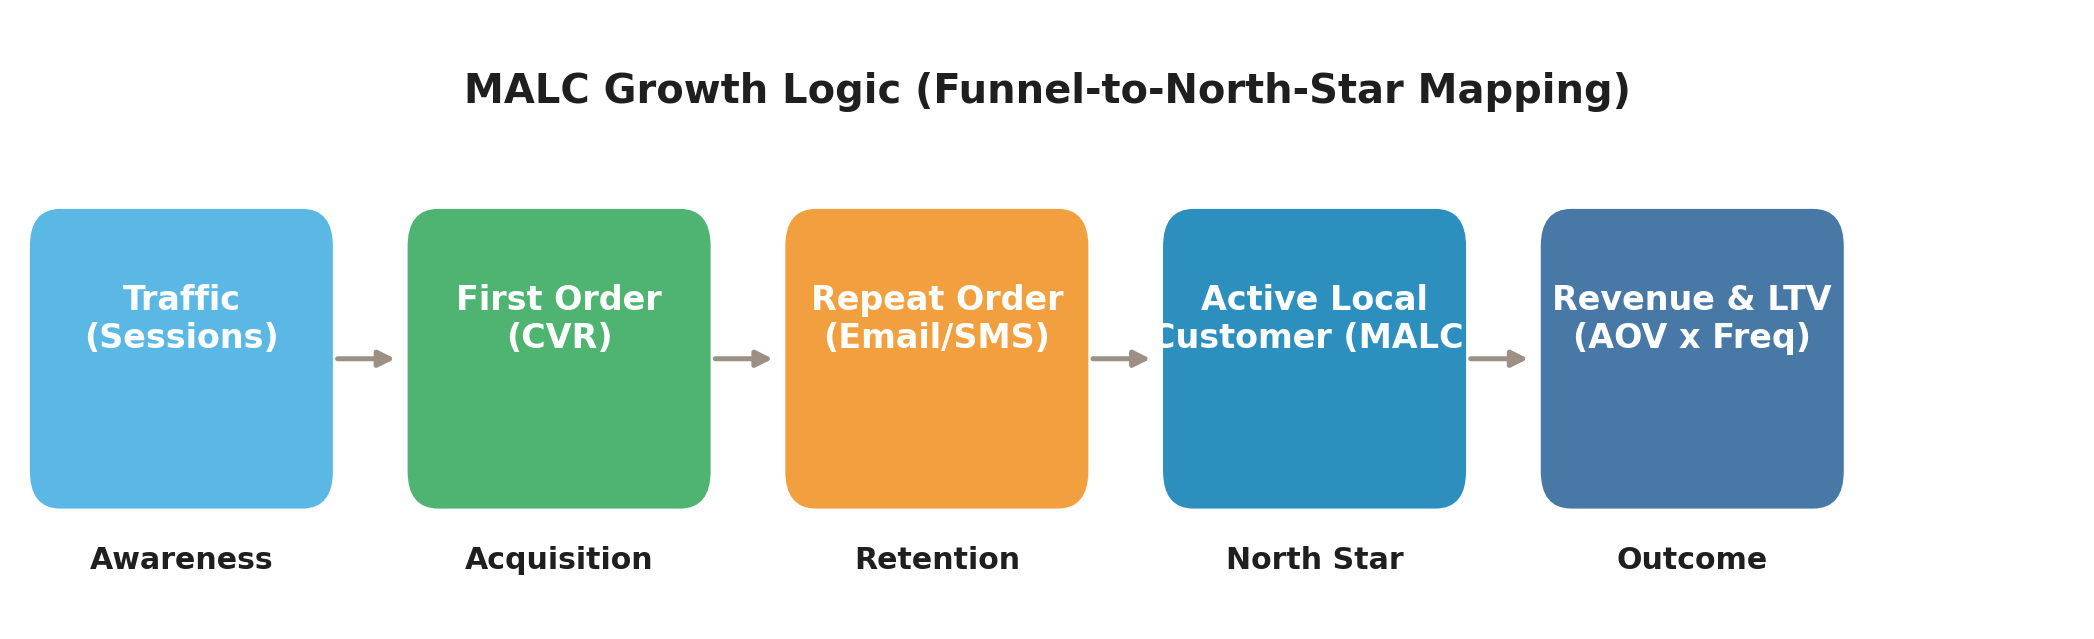
\includegraphics[width=0.95\linewidth]{figures/fig1_growth_logic} 

}

\caption{Figure 1: MALC growth logic, linking the funnel to the North Star and to long-term value.}\label{fig:unnamed-chunk-1}
\end{figure}

\subsubsection{SMART Objectives and KPI
Map}\label{smart-objectives-and-kpi-map}

Five SMART objectives drive MALC growth across the funnel. Each is tied
to a measurable KPI in the issued dataset (Table 1).

\begin{longtable}[]{@{}
  >{\raggedright\arraybackslash}p{(\linewidth - 8\tabcolsep) * \real{0.3475}}
  >{\raggedright\arraybackslash}p{(\linewidth - 8\tabcolsep) * \real{0.1780}}
  >{\raggedright\arraybackslash}p{(\linewidth - 8\tabcolsep) * \real{0.1525}}
  >{\raggedright\arraybackslash}p{(\linewidth - 8\tabcolsep) * \real{0.1017}}
  >{\raggedright\arraybackslash}p{(\linewidth - 8\tabcolsep) * \real{0.2203}}@{}}
\caption{SMART objectives mapped to KPIs and dataset
evidence.}\tabularnewline
\toprule\noalign{}
\begin{minipage}[b]{\linewidth}\raggedright
Objective
\end{minipage} & \begin{minipage}[b]{\linewidth}\raggedright
KPI
\end{minipage} & \begin{minipage}[b]{\linewidth}\raggedright
Target
\end{minipage} & \begin{minipage}[b]{\linewidth}\raggedright
Deadline
\end{minipage} & \begin{minipage}[b]{\linewidth}\raggedright
Evidence
\end{minipage} \\
\midrule\noalign{}
\endfirsthead
\toprule\noalign{}
\begin{minipage}[b]{\linewidth}\raggedright
Objective
\end{minipage} & \begin{minipage}[b]{\linewidth}\raggedright
KPI
\end{minipage} & \begin{minipage}[b]{\linewidth}\raggedright
Target
\end{minipage} & \begin{minipage}[b]{\linewidth}\raggedright
Deadline
\end{minipage} & \begin{minipage}[b]{\linewidth}\raggedright
Evidence
\end{minipage} \\
\midrule\noalign{}
\endhead
\bottomrule\noalign{}
\endlastfoot
Grow the local digital customer base & MALC & +60\% (430 → ≈690) & Feb
2027 & \texttt{malc} monthly \\
Improve site-wide conversion & CVR & ≥ 3.0\% & End Q3 2026 &
\texttt{orders/website\_sessions} \\
Build repeat revenue (subscriptions) & Active subscriptions & ≥ 700
active subs & End Q4 2026 & \texttt{active\_subscriptions} \\
Optimise paid efficiency & Blended ROAS & ≥ 1.5× blended & End Q2 2026 &
\texttt{revenue/total\_ad\_spend} \\
Build an owned marketing channel (email) & Email list size & ≥ 2,500
sign-ups & End Q2 2026 & \texttt{email\_signups} \\
\end{longtable}

\subsection{E-commerce MVP \& UX --- AI-Augmented
Shopify}\label{e-commerce-mvp-ux-ai-augmented-shopify}

\subsubsection{Platform choice and
rationale}\label{platform-choice-and-rationale}

Shopify Basic is recommended because it delivers (i) PCI-compliant
payments, SSL and GDPR cookie tooling out of the box; (ii) a mature app
ecosystem for subscription billing (Recharge), email (Klaviyo), and
accessibility (Accessibe); and (iii) a hosted Liquid theme that ships
natively as a mobile-first Progressive Web App (Shopify Inc., 2025).
Comparable monthly cost (\textasciitilde£29) and 2.0\% transaction fees
are within the founder's stated budget envelope.

WooCommerce is cheaper at face value but transfers infrastructure and
security responsibility onto the owner, who has limited technical
capacity (brief). Custom-build is out of scope on time and risk grounds.

\subsubsection{AI-driven MVP
architecture}\label{ai-driven-mvp-architecture}

The MVP layers a thin AI decisioning tier on top of Shopify (Figure 8).
The LLM-powered recommendation engine personalises the product feed
using the order history; Prophet (Taylor \& Letham, 2018) forecasts
demand to drive baking quantities; a gradient-boosted churn model flags
at-risk subscribers into a Klaviyo win-back flow; and a GenAI content
studio drafts menu copy, ALT text and social captions for founder
review.

\begin{figure}

{\centering 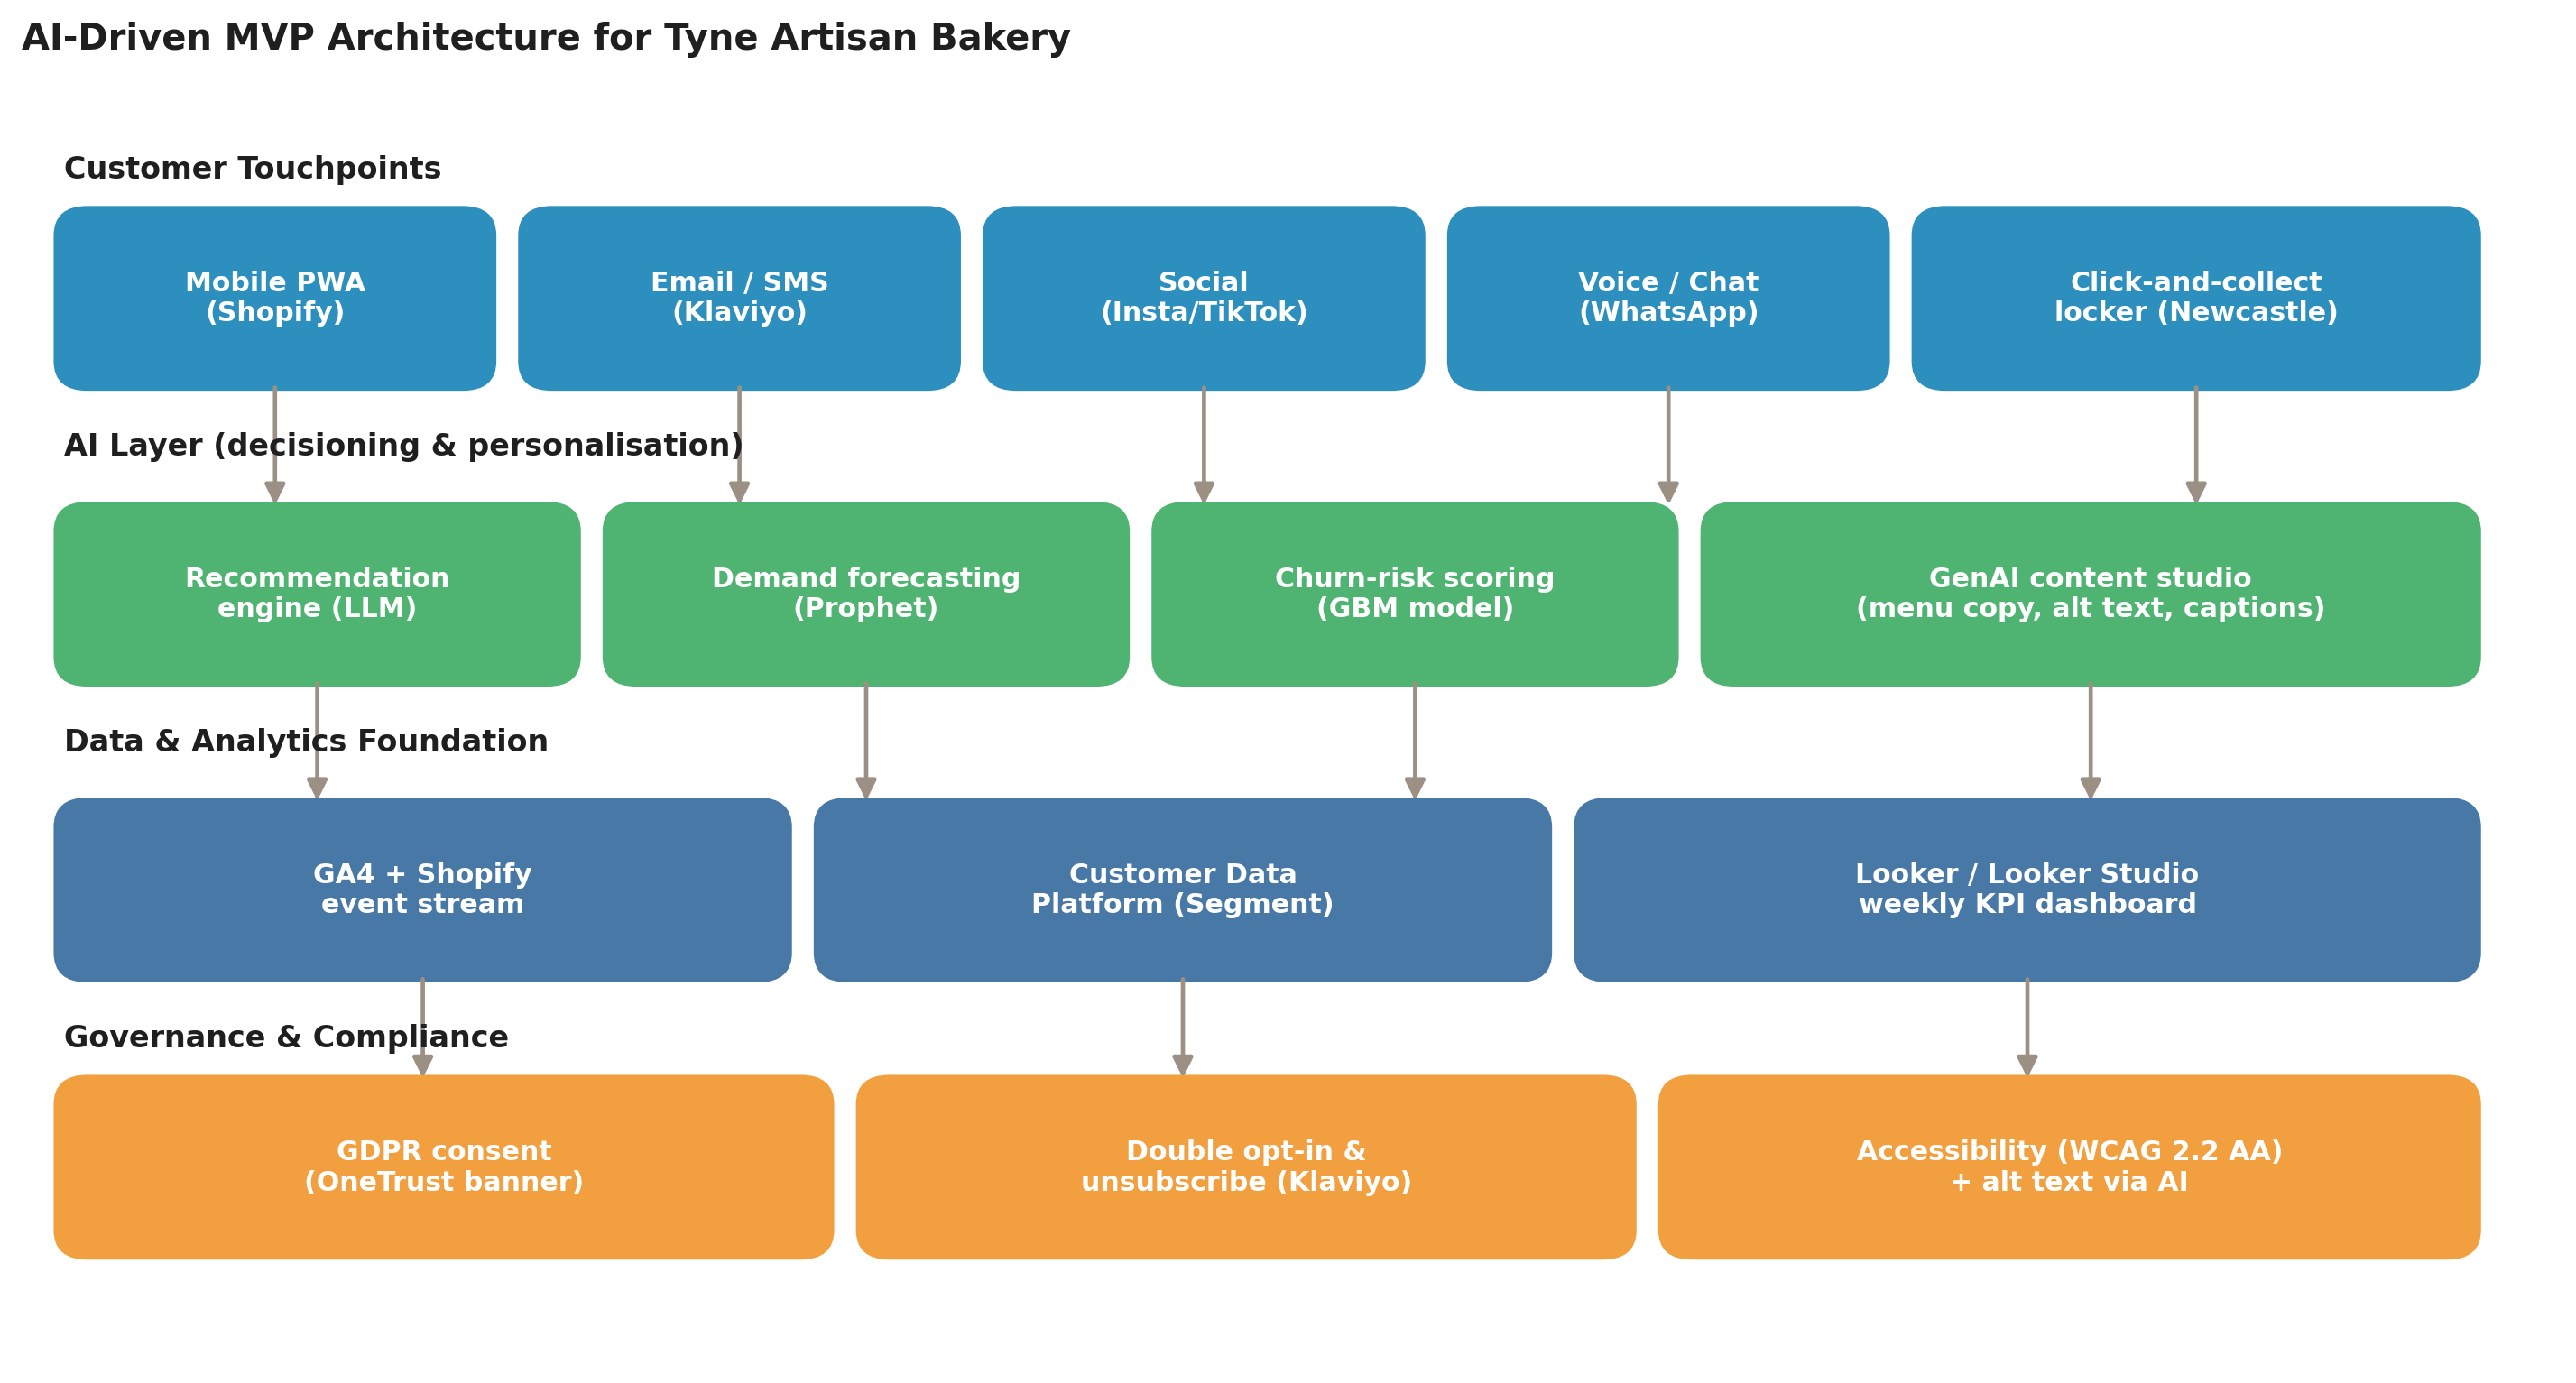
\includegraphics[width=0.95\linewidth]{figures/fig8_ai_mvp_architecture} 

}

\caption{Figure 8: AI-Augmented MVP Architecture. Customer touchpoints feed an AI decisioning layer, which is grounded by a measurement foundation and wrapped in a governance ring.}\label{fig:unnamed-chunk-3}
\end{figure}

\subsubsection{Information Architecture}\label{information-architecture}

The information architecture is deliberately shallow (max three clicks
to purchase). The site map (Figure 10) consolidates discovery under
\texttt{Shop}, recurring revenue under \texttt{Subscription}, and trust
artefacts (privacy, returns, accessibility, allergens) into a single
footer cluster --- a pattern shown to reduce checkout abandonment
(Baymard Institute, 2024).

\begin{figure}

{\centering 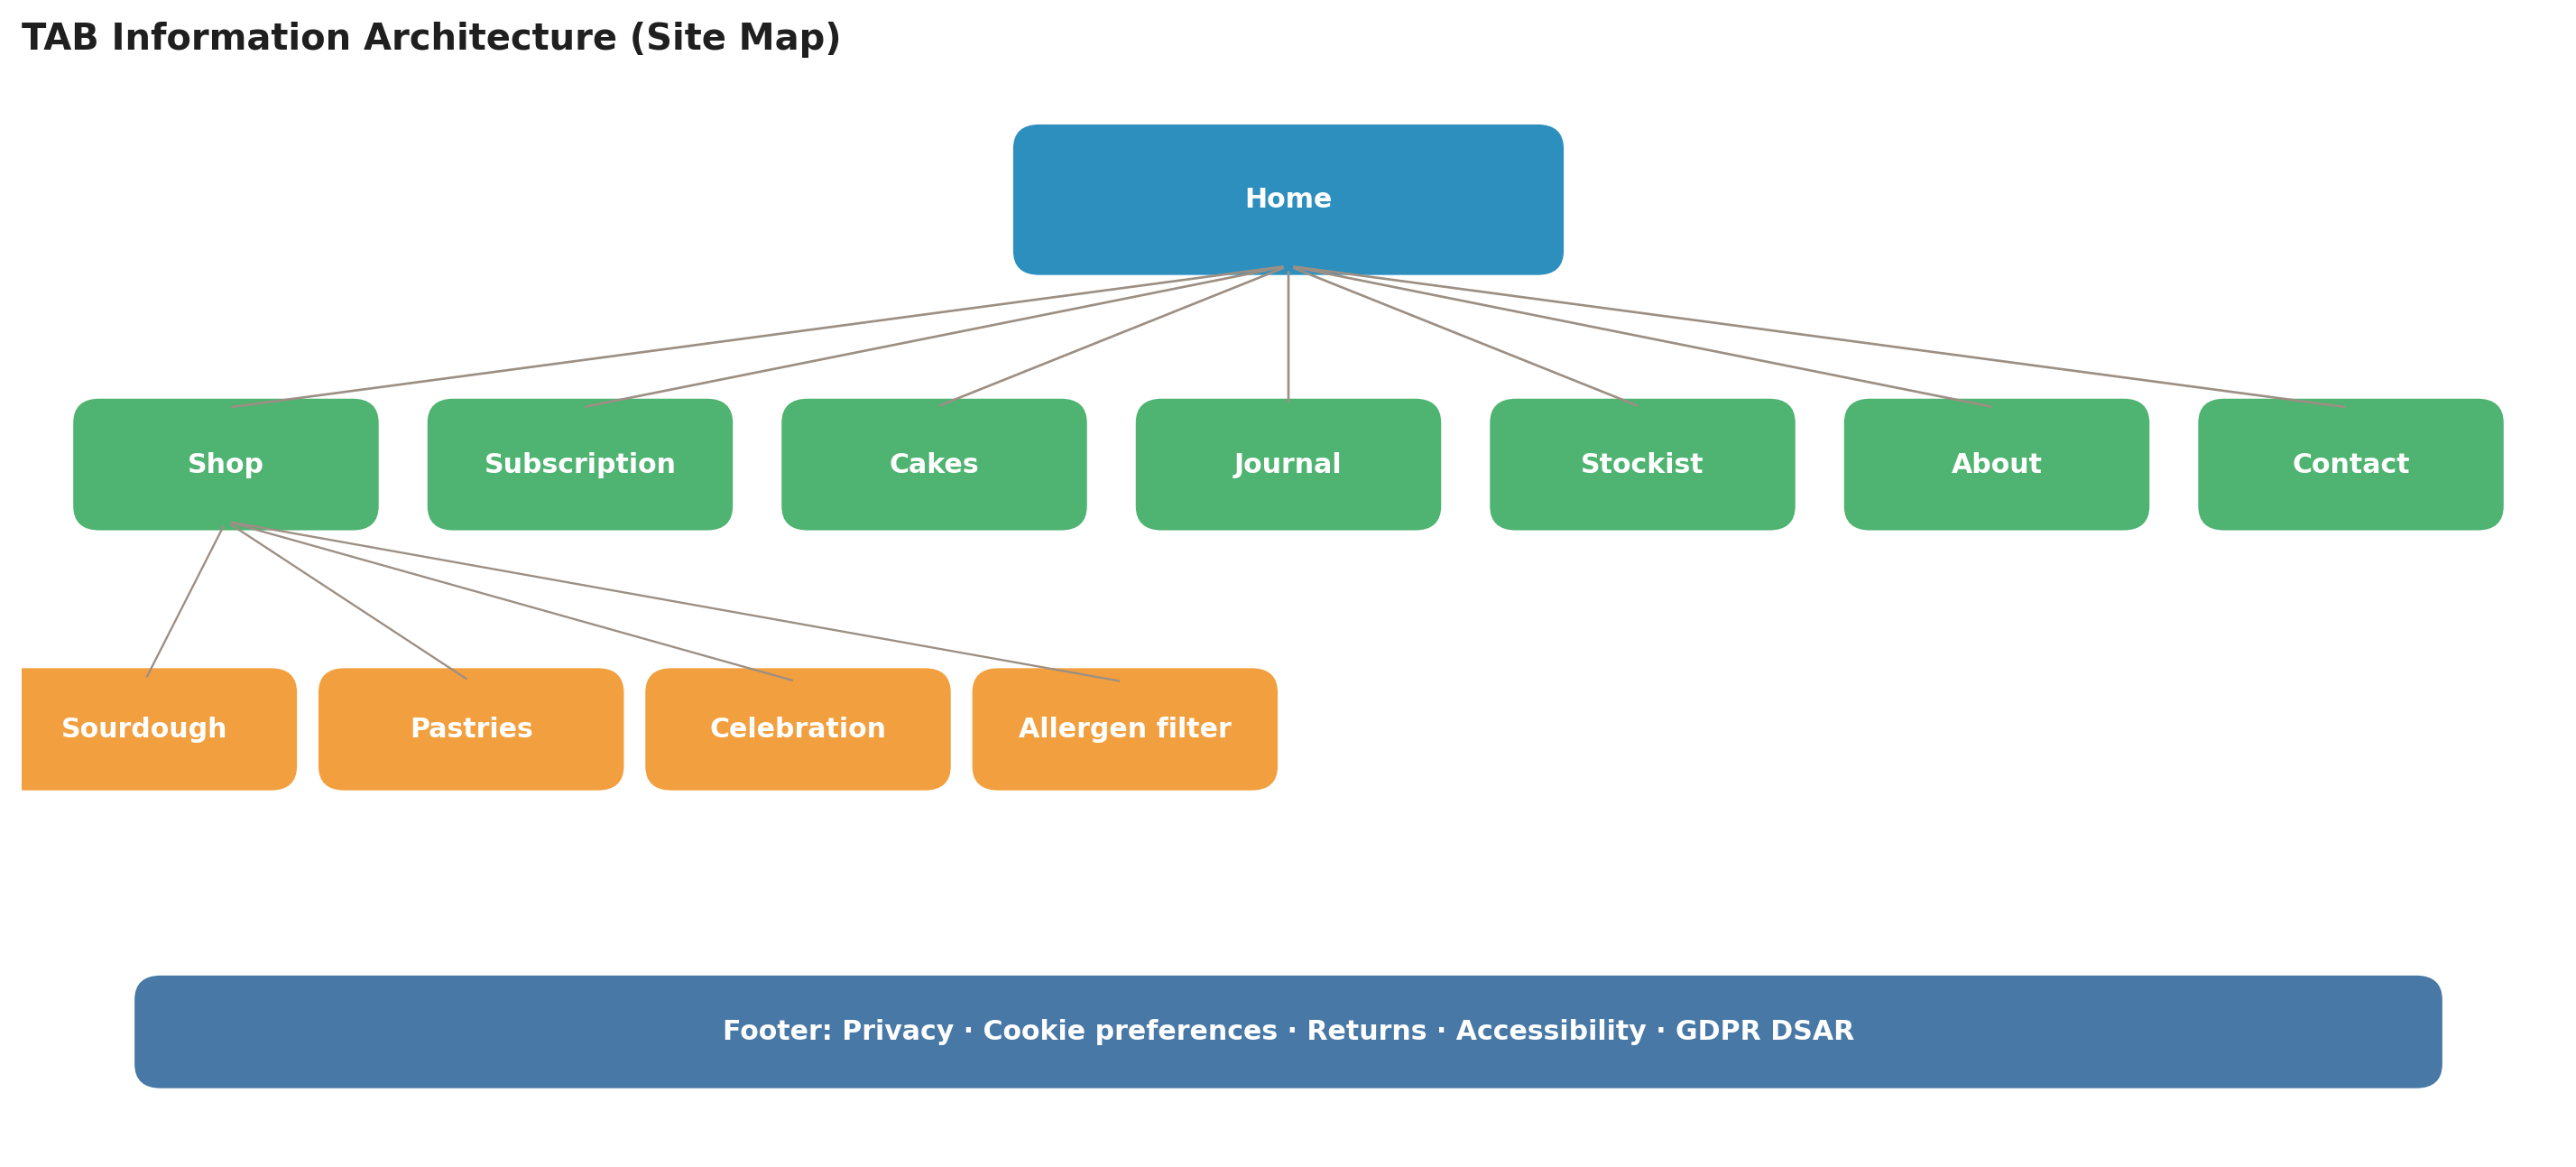
\includegraphics[width=0.95\linewidth]{figures/fig10_site_map} 

}

\caption{Figure 10: TAB information architecture (site map).}\label{fig:unnamed-chunk-4}
\end{figure}

\subsubsection{UX Wireframes}\label{ux-wireframes}

Three mobile screens are wireframed (Figure 9). Each is built to
PDP-best-practice principles: above-the-fold imagery, social proof,
allergen disclosure, delivery slot picker, and an explicit subscription
cross-sell. The single-page checkout exposes Apple Pay and Google Pay
first because mobile express-wallet adoption shortens purchase paths by
35--45\% in DTC food categories (Stripe, 2025).

\begin{figure}

{\centering 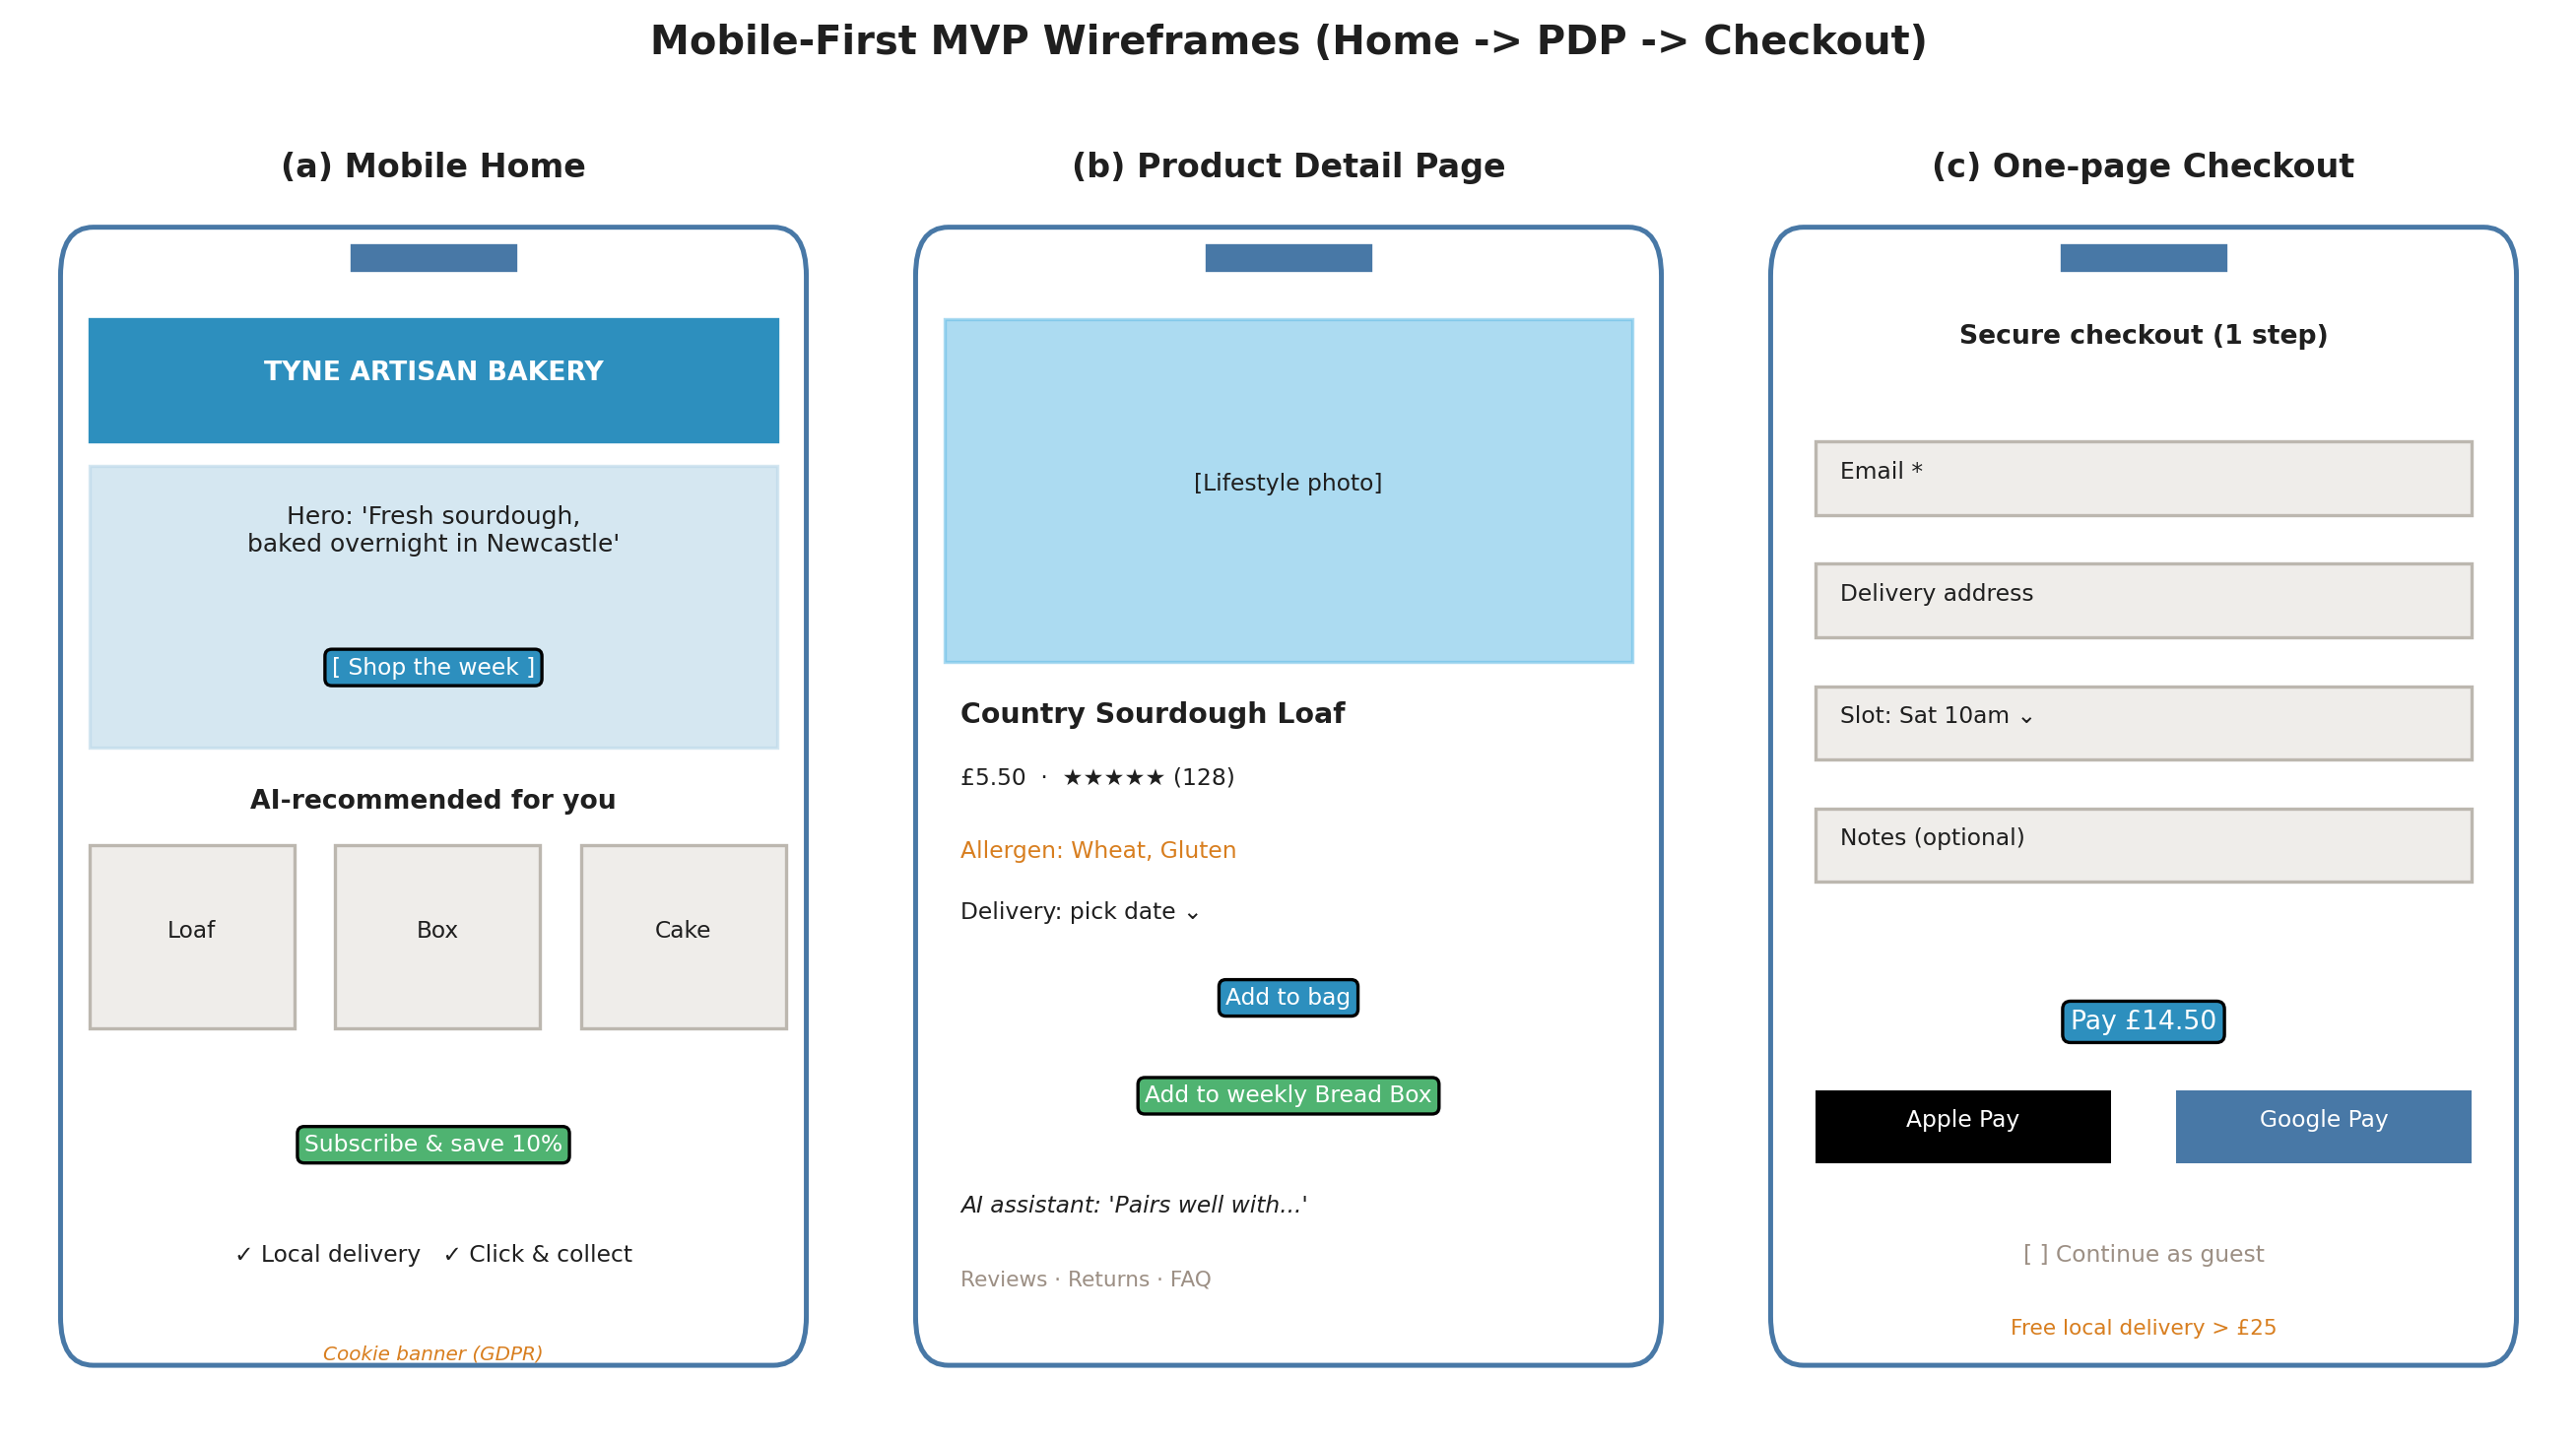
\includegraphics[width=0.95\linewidth]{figures/fig9_ux_wireframes} 

}

\caption{Figure 9: Mobile-first MVP wireframes — Home / PDP / Checkout. Each frame embeds AI personalisation and a GDPR-compliant footer.}\label{fig:unnamed-chunk-5}
\end{figure}

\subsection{Channel \& Content Strategy}\label{channel-content-strategy}

\subsubsection{Personas and funnel
mapping}\label{personas-and-funnel-mapping}

Three evidence-based personas emerge from the order data: a
\textbf{Weekly Bread Buyer} (high subscription share, low AOV variance),
a \textbf{Celebration Cake Buyer} (high AOV, event-driven), and a
\textbf{Weekend Treat Buyer} (mobile, impulse, low subscription
affinity). Their journeys differ across the funnel and so do the
appropriate content vehicles (Figure 7).

\begin{figure}

{\centering 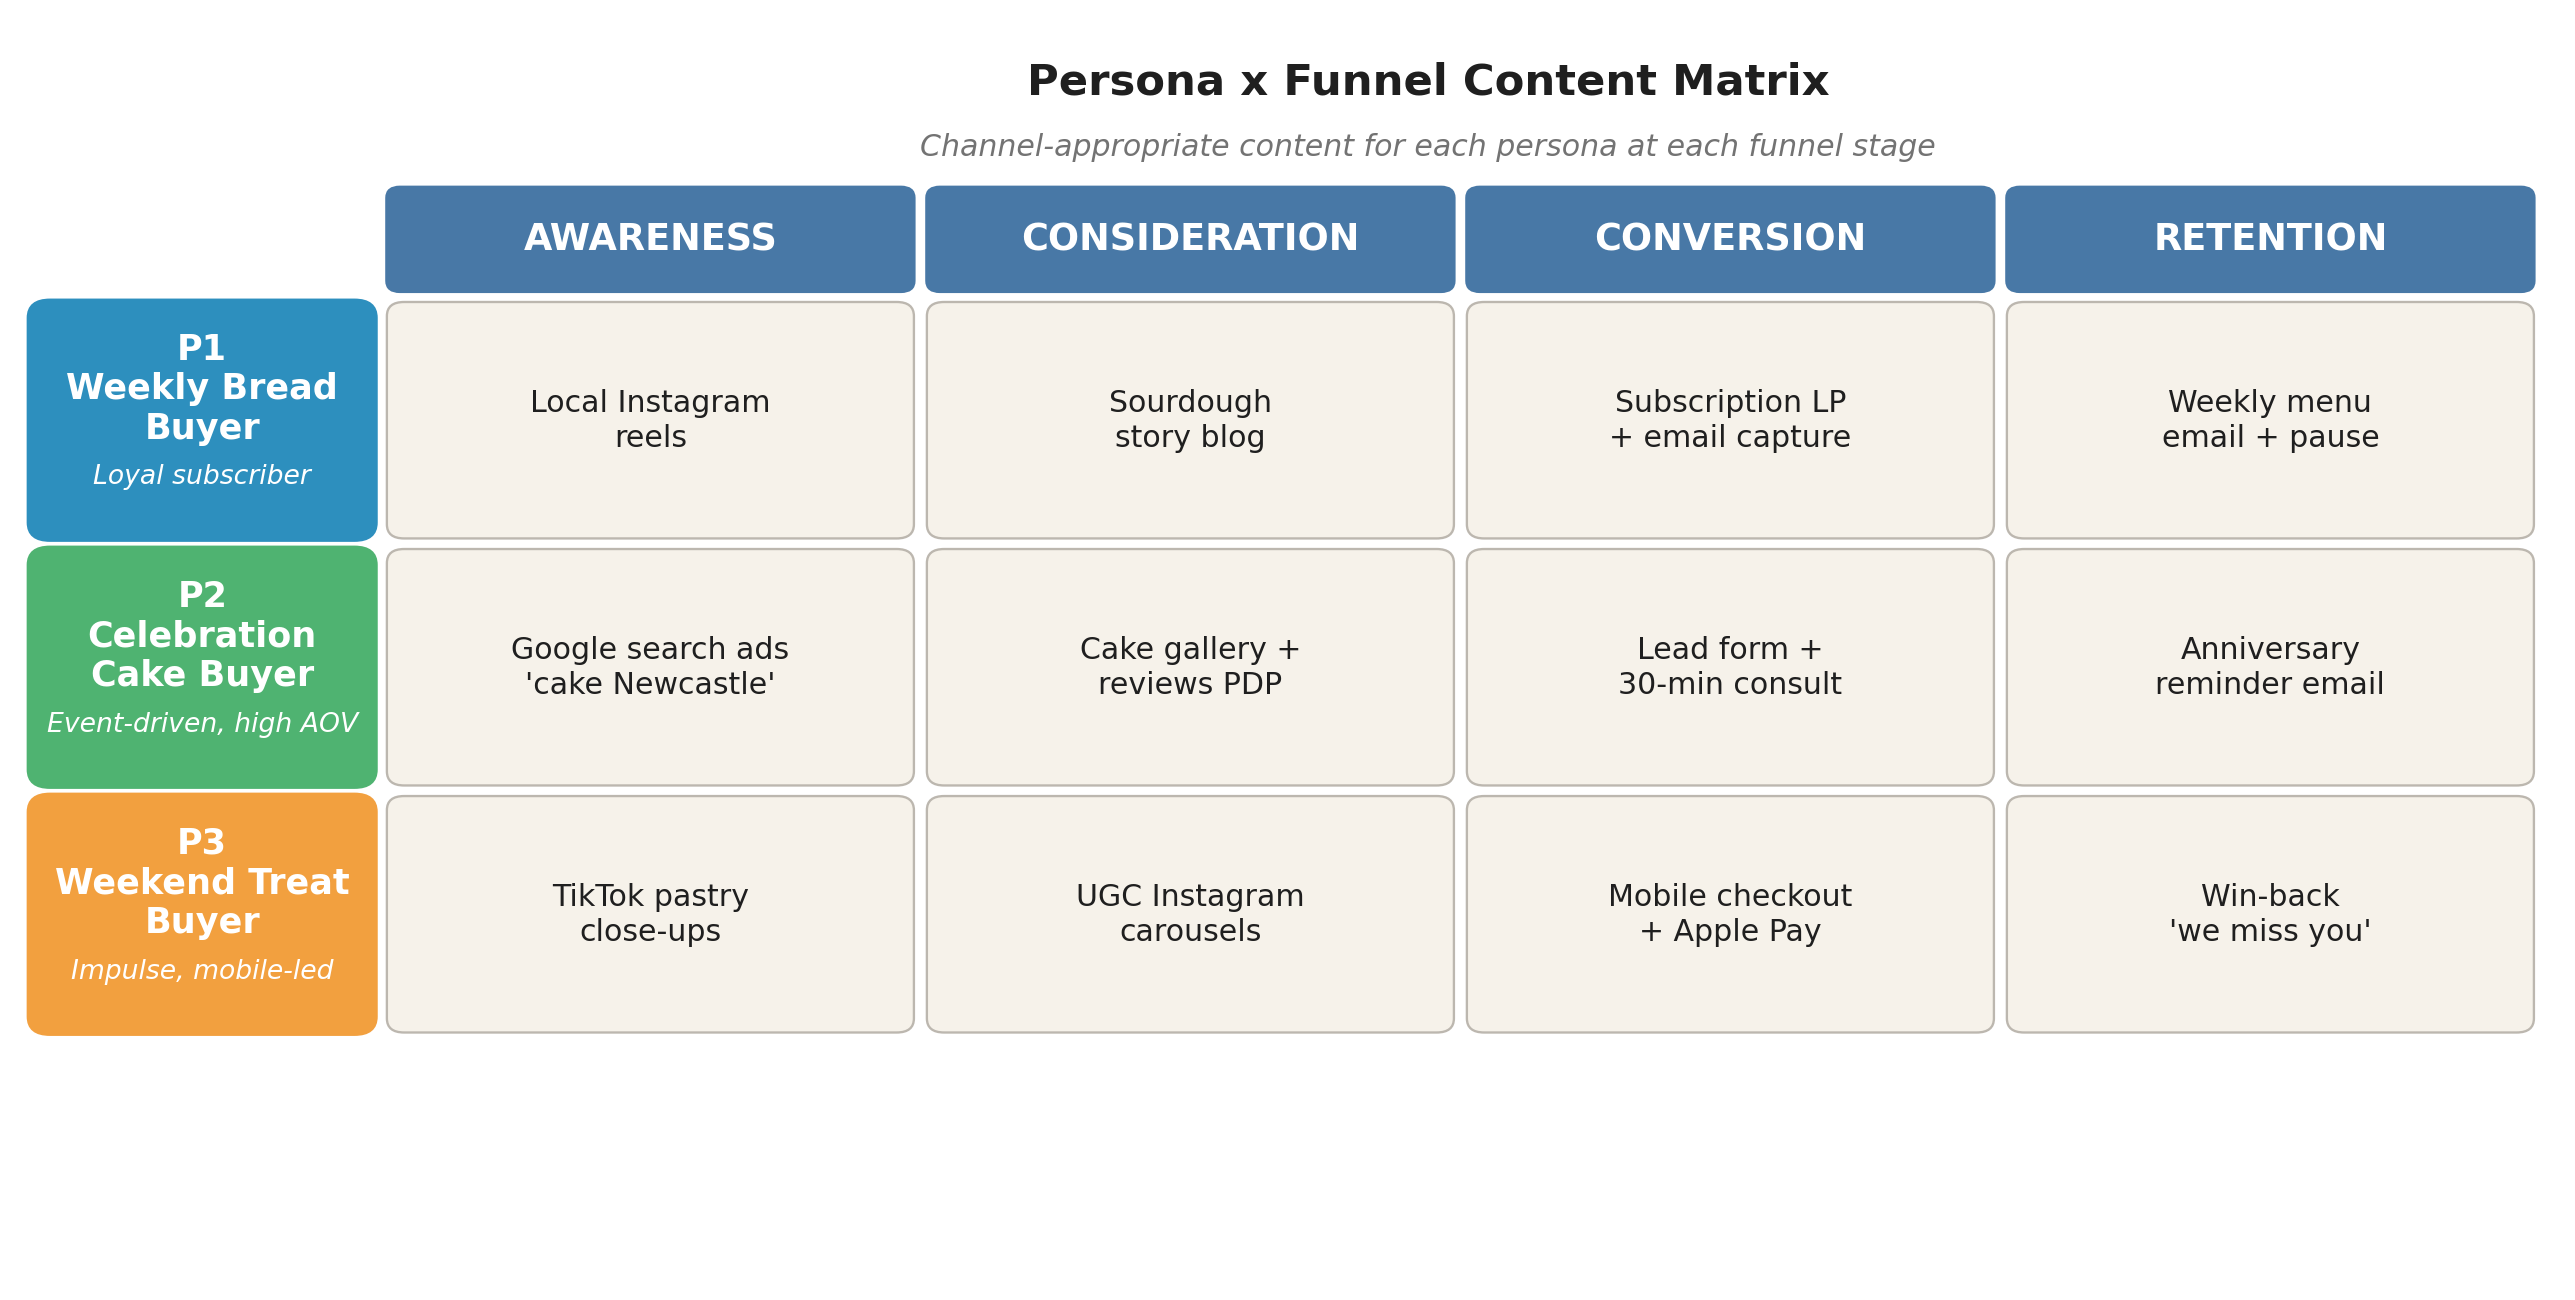
\includegraphics[width=0.95\linewidth]{figures/fig7_persona_funnel} 

}

\caption{Figure 7: Persona × Funnel content matrix. Each cell pairs a persona with channel-appropriate content for that funnel stage.}\label{fig:unnamed-chunk-6}
\end{figure}

\subsubsection{Budget allocation (paid)}\label{budget-allocation-paid}

The recommended split between Google, Meta and TikTok (Q1 baseline) is
\textbf{60 / 25 / 15} because Google is the only paid channel that
currently breaks even (§2.5). This is \textbf{inverted} from a typical
DTC-food split where Meta dominates, but is the right policy given TAB's
high-intent product (branded local search) and the observed ROAS data.
The split is revisited quarterly using the rule in §2.6.3.

\subsubsection{Content pillars and
cadence}\label{content-pillars-and-cadence}

Four content pillars are proposed, each mapped to a SMART KPI:

\begin{longtable}[]{@{}
  >{\raggedright\arraybackslash}p{(\linewidth - 6\tabcolsep) * \real{0.2500}}
  >{\raggedright\arraybackslash}p{(\linewidth - 6\tabcolsep) * \real{0.2500}}
  >{\raggedright\arraybackslash}p{(\linewidth - 6\tabcolsep) * \real{0.2500}}
  >{\raggedright\arraybackslash}p{(\linewidth - 6\tabcolsep) * \real{0.2500}}@{}}
\toprule\noalign{}
\begin{minipage}[b]{\linewidth}\raggedright
Pillar
\end{minipage} & \begin{minipage}[b]{\linewidth}\raggedright
Cadence
\end{minipage} & \begin{minipage}[b]{\linewidth}\raggedright
Lead format
\end{minipage} & \begin{minipage}[b]{\linewidth}\raggedright
Primary KPI
\end{minipage} \\
\midrule\noalign{}
\endhead
\bottomrule\noalign{}
\endlastfoot
Craft \& process (sourdough school, fermentation, bakers' stories) & 2 ×
Instagram Reel + 1 × TikTok / week & Short video & Followers; CTR to
site \\
Weekly menu drop & 1 × email + 1 × Instagram Story / week & Email +
carousel & Email-attributed CVR \\
Allergen \& education & 1 × blog / month & Long-form SEO & Organic
sessions, dwell time \\
Local community & Monthly micro-influencer activation & UGC / Reels &
Social engagements, MALC NE \\
\end{longtable}

\subsubsection{Experimentation roadmap}\label{experimentation-roadmap}

A continuous-testing programme is proposed (Kohavi, Tang \& Xu, 2020).
Each test runs to a pre-registered minimum detectable effect (MDE) of
10\% with α = 0.05 and 80\% power. The hero-banner test in this report
is the first; follow-ups include (a) free-delivery threshold (£25 vs
£35), (b) subscription discount band (5\% vs 10\%), and (c) PDP layout
(image-first vs reviews-first).

\subsection{Analytics \& Measurement}\label{analytics-measurement}

A weekly cadence with quarterly reallocation is the right rhythm for a
microenterprise (Croll \& Yoskovitz, 2013). The governance flow in
Figure 14 codifies who owns what.

\begin{figure}

{\centering 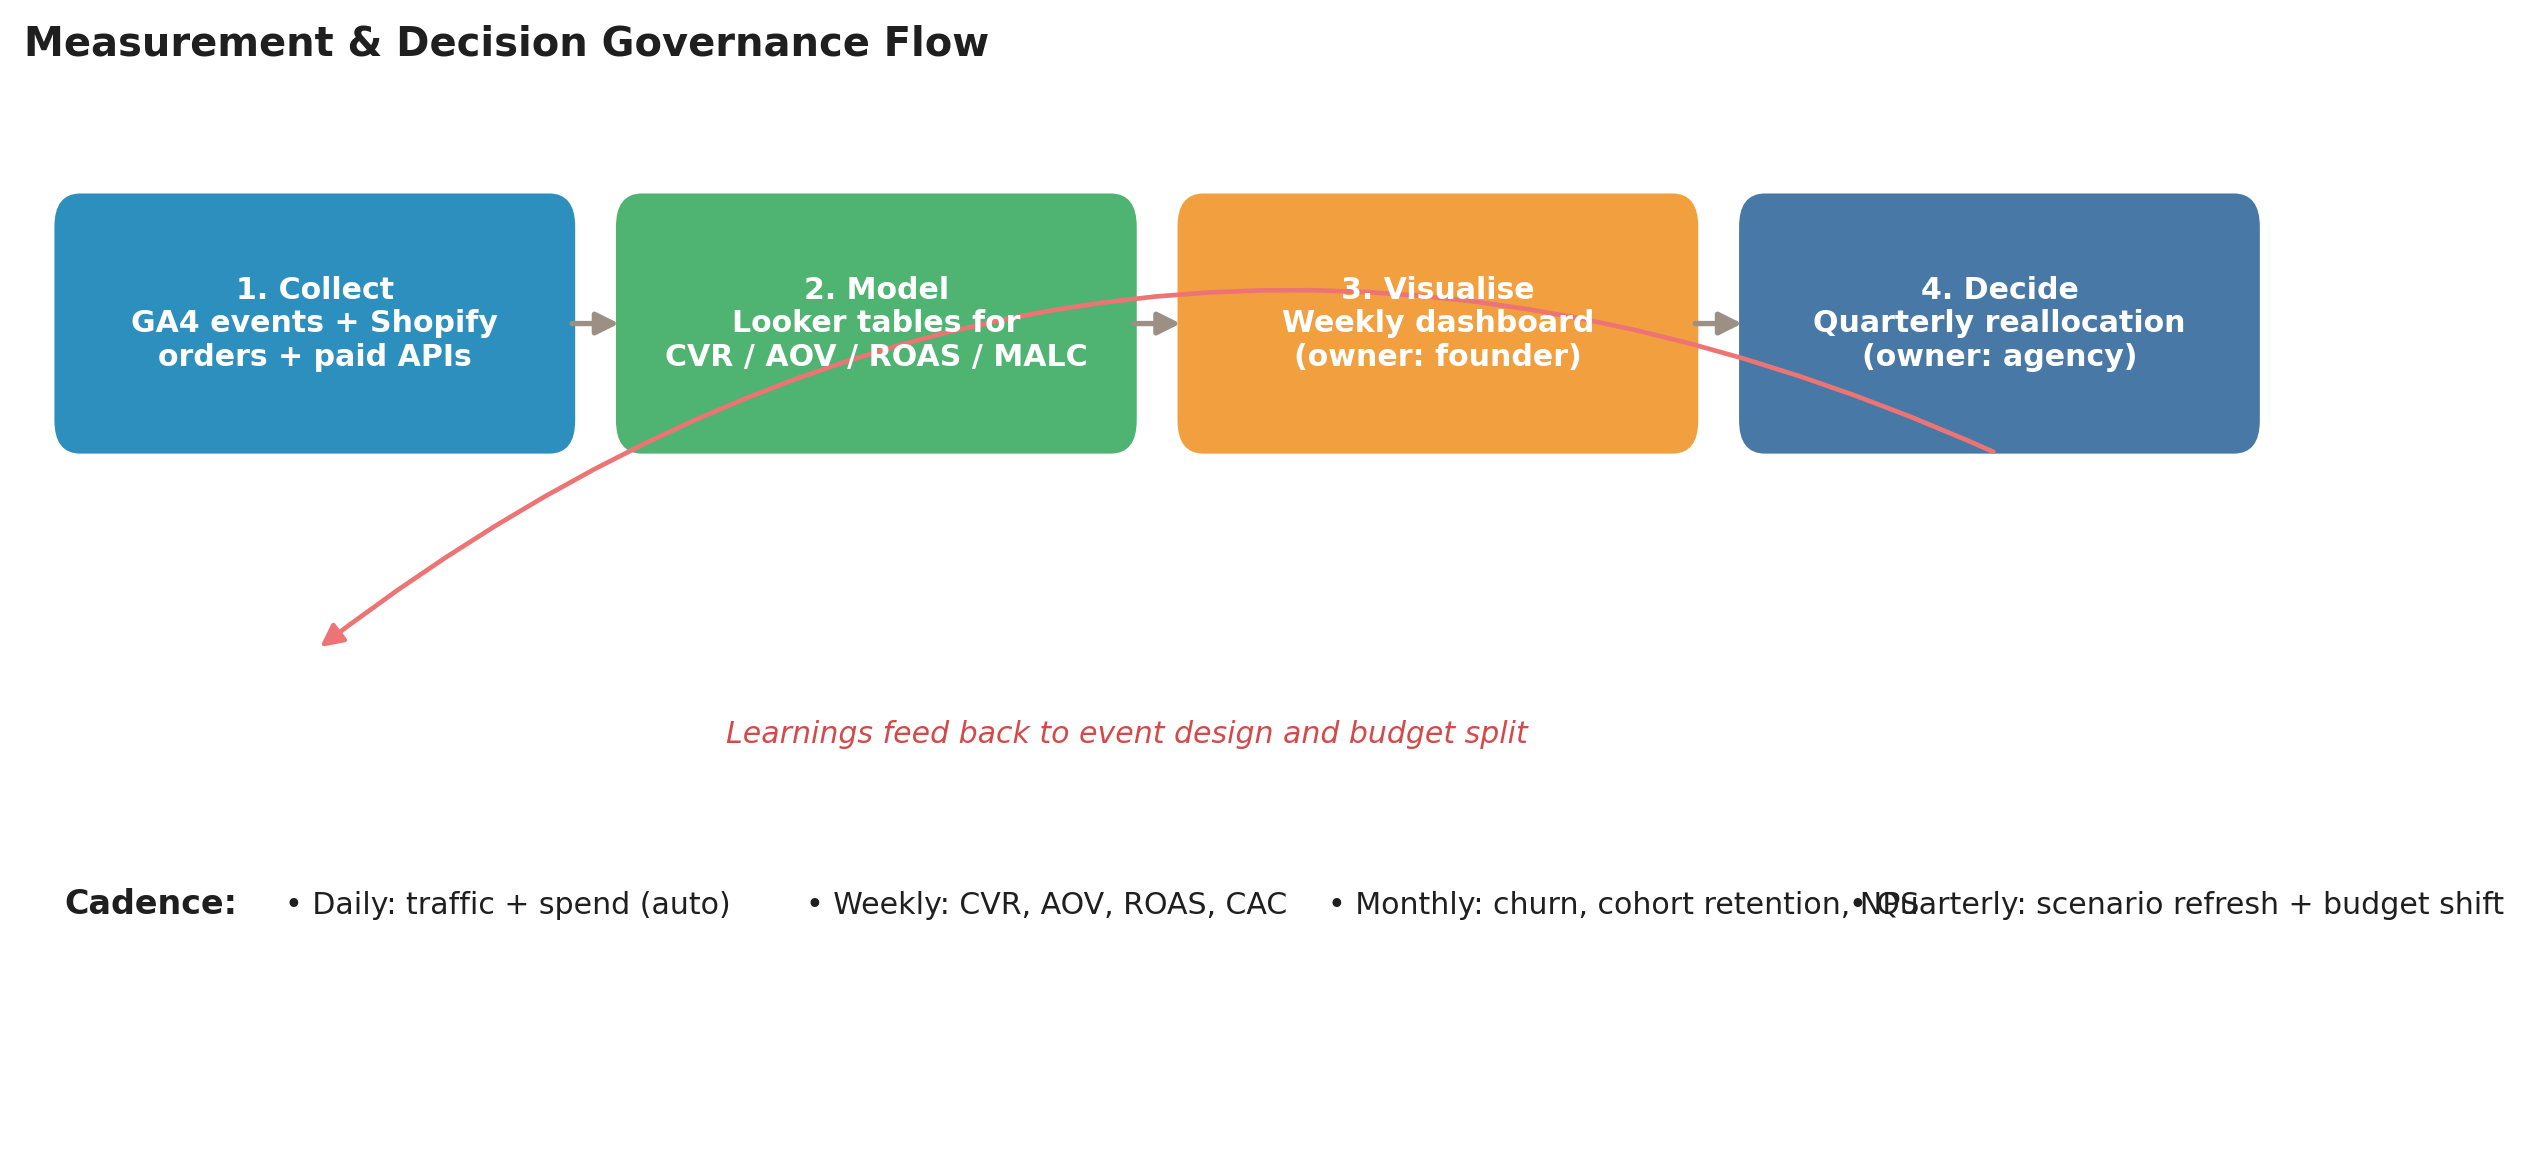
\includegraphics[width=0.95\linewidth]{figures/fig14_governance} 

}

\caption{Figure 14: Measurement and decision governance flow. Data is collected daily, modelled into weekly KPIs, visualised in a single dashboard, and converted into quarterly budget decisions.}\label{fig:unnamed-chunk-7}
\end{figure}

\subsubsection{Dashboard specification}\label{dashboard-specification}

\begin{longtable}[]{@{}
  >{\raggedright\arraybackslash}p{(\linewidth - 10\tabcolsep) * \real{0.1203}}
  >{\raggedright\arraybackslash}p{(\linewidth - 10\tabcolsep) * \real{0.2632}}
  >{\raggedright\arraybackslash}p{(\linewidth - 10\tabcolsep) * \real{0.1805}}
  >{\raggedright\arraybackslash}p{(\linewidth - 10\tabcolsep) * \real{0.0602}}
  >{\raggedright\arraybackslash}p{(\linewidth - 10\tabcolsep) * \real{0.1278}}
  >{\raggedright\arraybackslash}p{(\linewidth - 10\tabcolsep) * \real{0.2481}}@{}}
\caption{Weekly dashboard specification with owners, cadence and action
thresholds.}\tabularnewline
\toprule\noalign{}
\begin{minipage}[b]{\linewidth}\raggedright
Tile
\end{minipage} & \begin{minipage}[b]{\linewidth}\raggedright
Metrics
\end{minipage} & \begin{minipage}[b]{\linewidth}\raggedright
Tools
\end{minipage} & \begin{minipage}[b]{\linewidth}\raggedright
Cadence
\end{minipage} & \begin{minipage}[b]{\linewidth}\raggedright
Owner
\end{minipage} & \begin{minipage}[b]{\linewidth}\raggedright
Action threshold
\end{minipage} \\
\midrule\noalign{}
\endfirsthead
\toprule\noalign{}
\begin{minipage}[b]{\linewidth}\raggedright
Tile
\end{minipage} & \begin{minipage}[b]{\linewidth}\raggedright
Metrics
\end{minipage} & \begin{minipage}[b]{\linewidth}\raggedright
Tools
\end{minipage} & \begin{minipage}[b]{\linewidth}\raggedright
Cadence
\end{minipage} & \begin{minipage}[b]{\linewidth}\raggedright
Owner
\end{minipage} & \begin{minipage}[b]{\linewidth}\raggedright
Action threshold
\end{minipage} \\
\midrule\noalign{}
\endhead
\bottomrule\noalign{}
\endlastfoot
Acquisition & Sessions, users, share by channel & GA4 + Looker Studio &
Weekly & Founder & Organic share \textless{} 30\% ⇒ SEO push \\
Conversion & CVR, AOV, cart-abandonment & GA4 + Shopify & Weekly &
Founder & CVR \textless{} 2.5\% ⇒ run next A/B test \\
Paid efficiency & Spend, ROAS, CAC by platform & Google/Meta/TikTok APIs
& Weekly & Agency / founder & ROAS \textless{} 1.0× ⇒ pause / cut
budget \\
Retention & Active subs, churn, repeat rate & Klaviyo + Shopify & Weekly
& Founder & Churn \textgreater{} 5\% ⇒ launch win-back \\
Content & Posts, engagements, clicks to site & Meta/TikTok APIs & Weekly
& Social assistant & Engagement \textless{} 2\% ⇒ pillar review \\
\end{longtable}

\subsection{Data Analysis --- Key
Insights}\label{data-analysis-key-insights}

\subsubsection{MALC and revenue trend}\label{malc-and-revenue-trend}

The blended MALC and revenue series (Figure 2) shows a noisy but clearly
positive trajectory: from \textbf{92 customers in March 2024} to
\textbf{430 in February 2026} (the last complete month in the dataset; a
partial March 2026 is excluded from the trend to avoid bias). The
compound monthly MALC growth across the trailing twelve months is
approximately \textbf{4.0\%}, which is what anchors the \emph{Base}
forecast scenario in §2.6.

\begin{figure}

{\centering 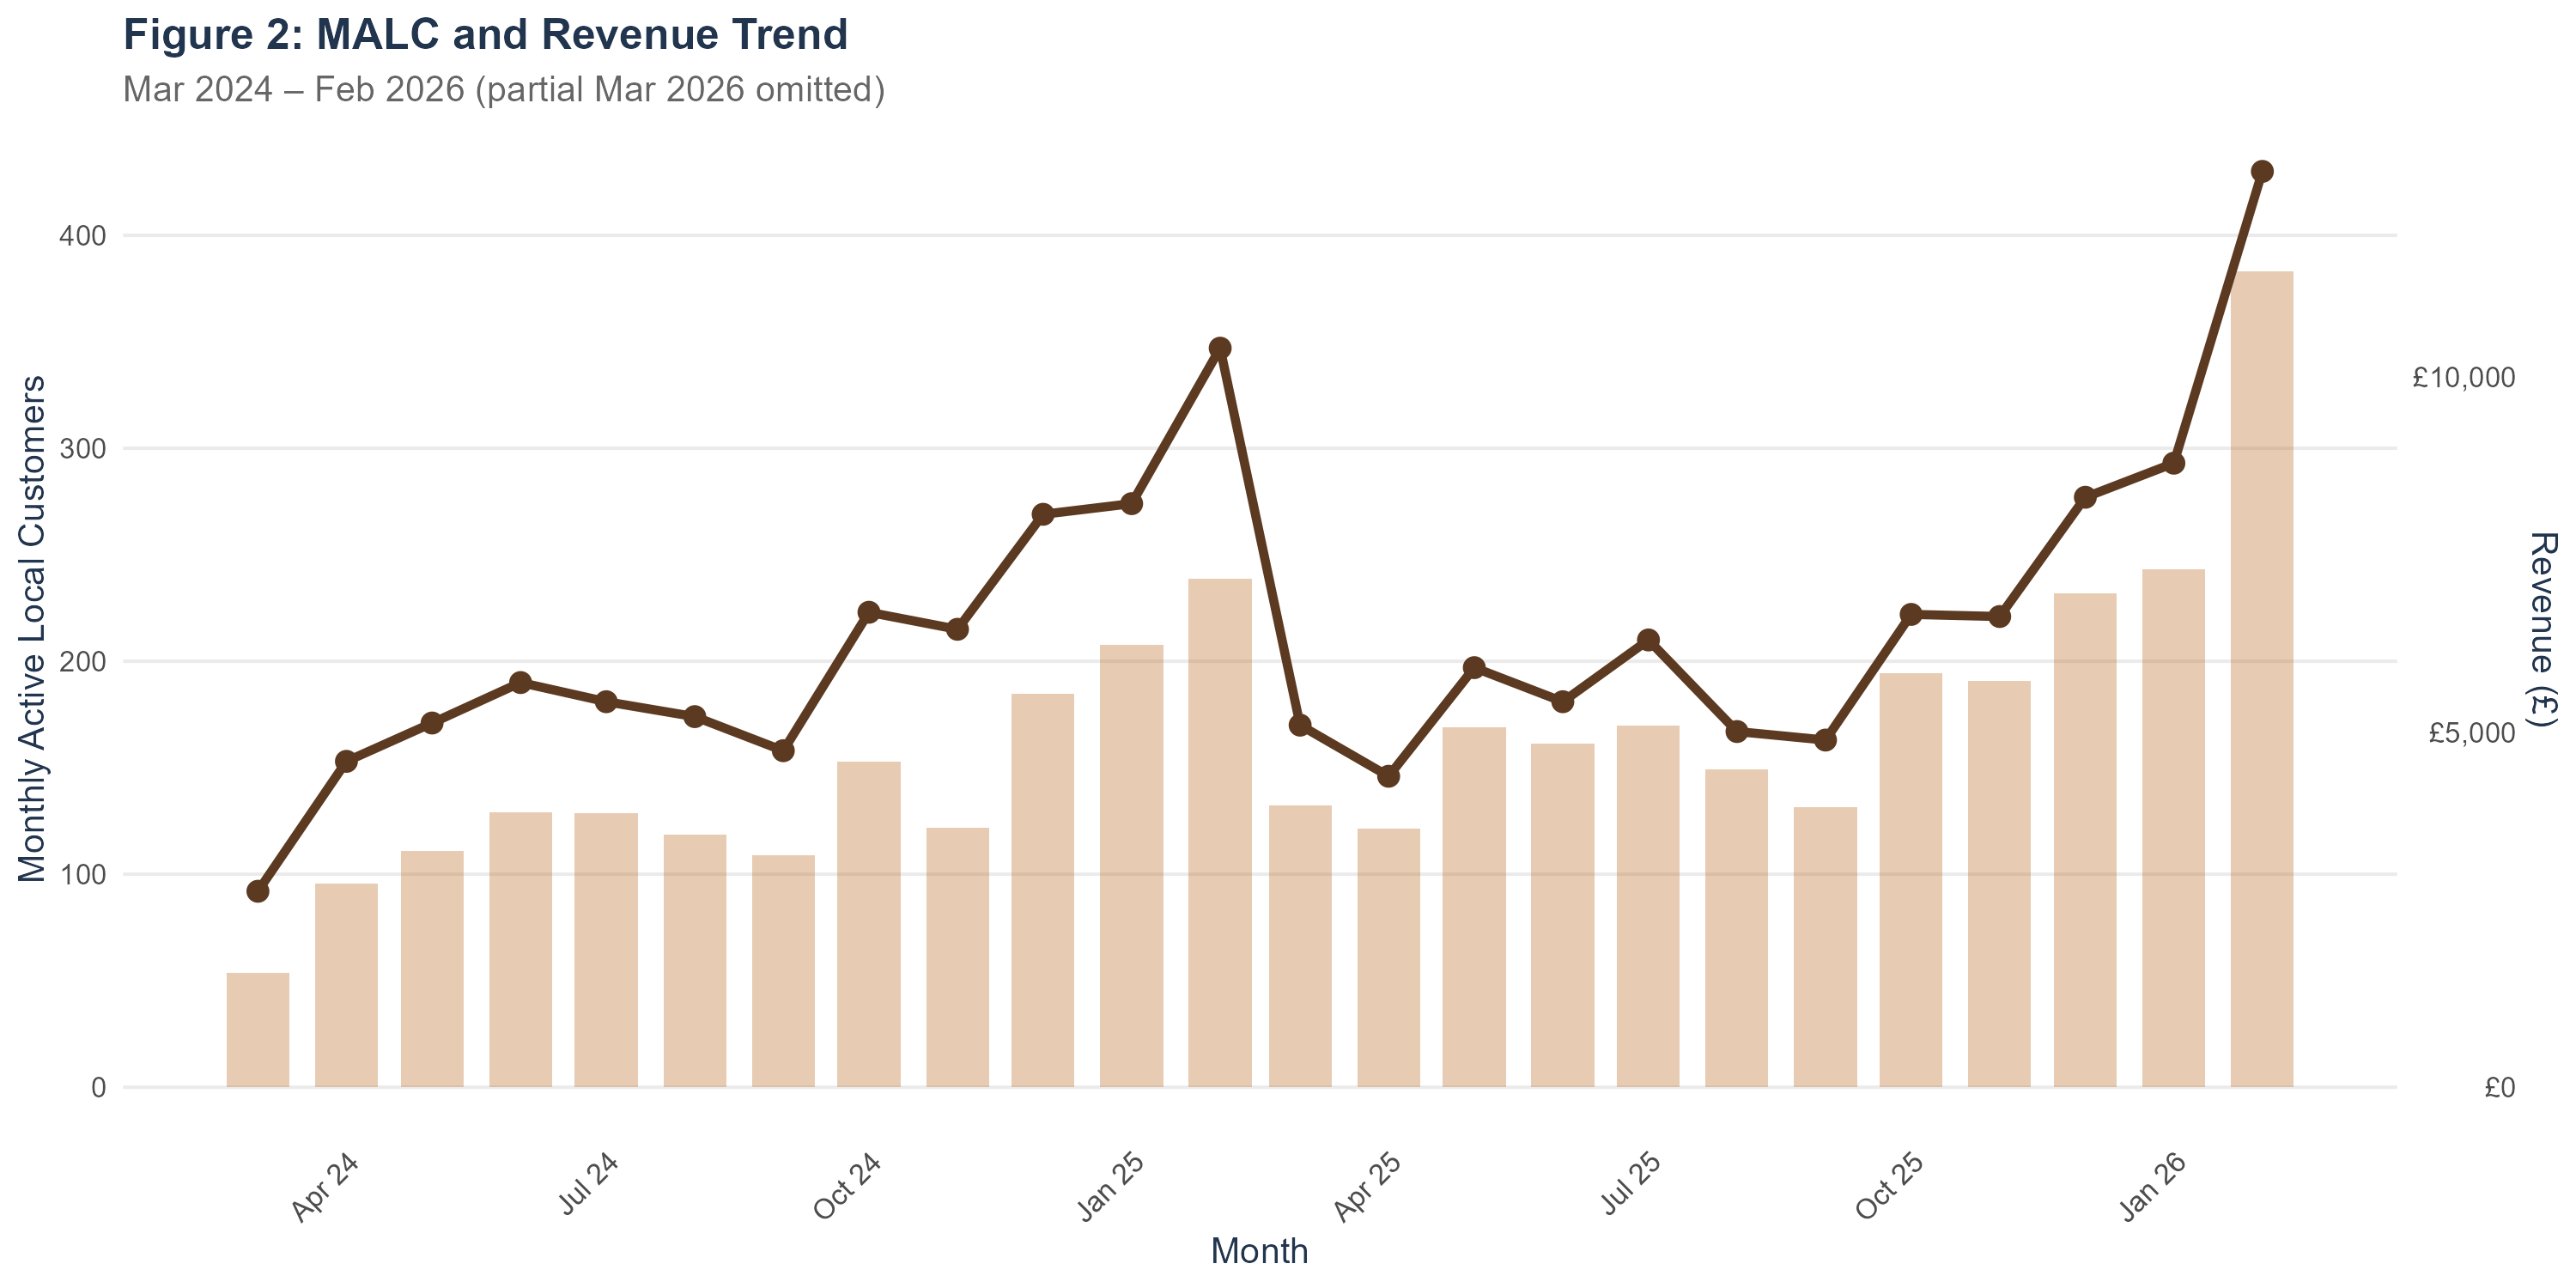
\includegraphics[width=0.95\linewidth]{figures/fig2_malc_revenue_trend} 

}

\caption{Figure 2: MALC and revenue trend. Bars show revenue (right axis); the brown line shows MALC (left axis).}\label{fig:unnamed-chunk-9}
\end{figure}

\subsubsection{Paid channel efficiency --- the unprofitability
finding}\label{paid-channel-efficiency-the-unprofitability-finding}

The critical analytical finding of the report is that \textbf{only
Google search is profitable on a last-click attribution basis} (Figure
3). Across the full window, blended CAC (£36--£52) exceeds AOV (£20.34)
on every paid platform. The implication is structural: TAB cannot grow
profitably through paid alone; the plan must lead with owned channels
(email, subscriptions) and SEO, and treat paid as a controlled
experiment until ROAS clears 1.0× consistently.

\begin{figure}

{\centering 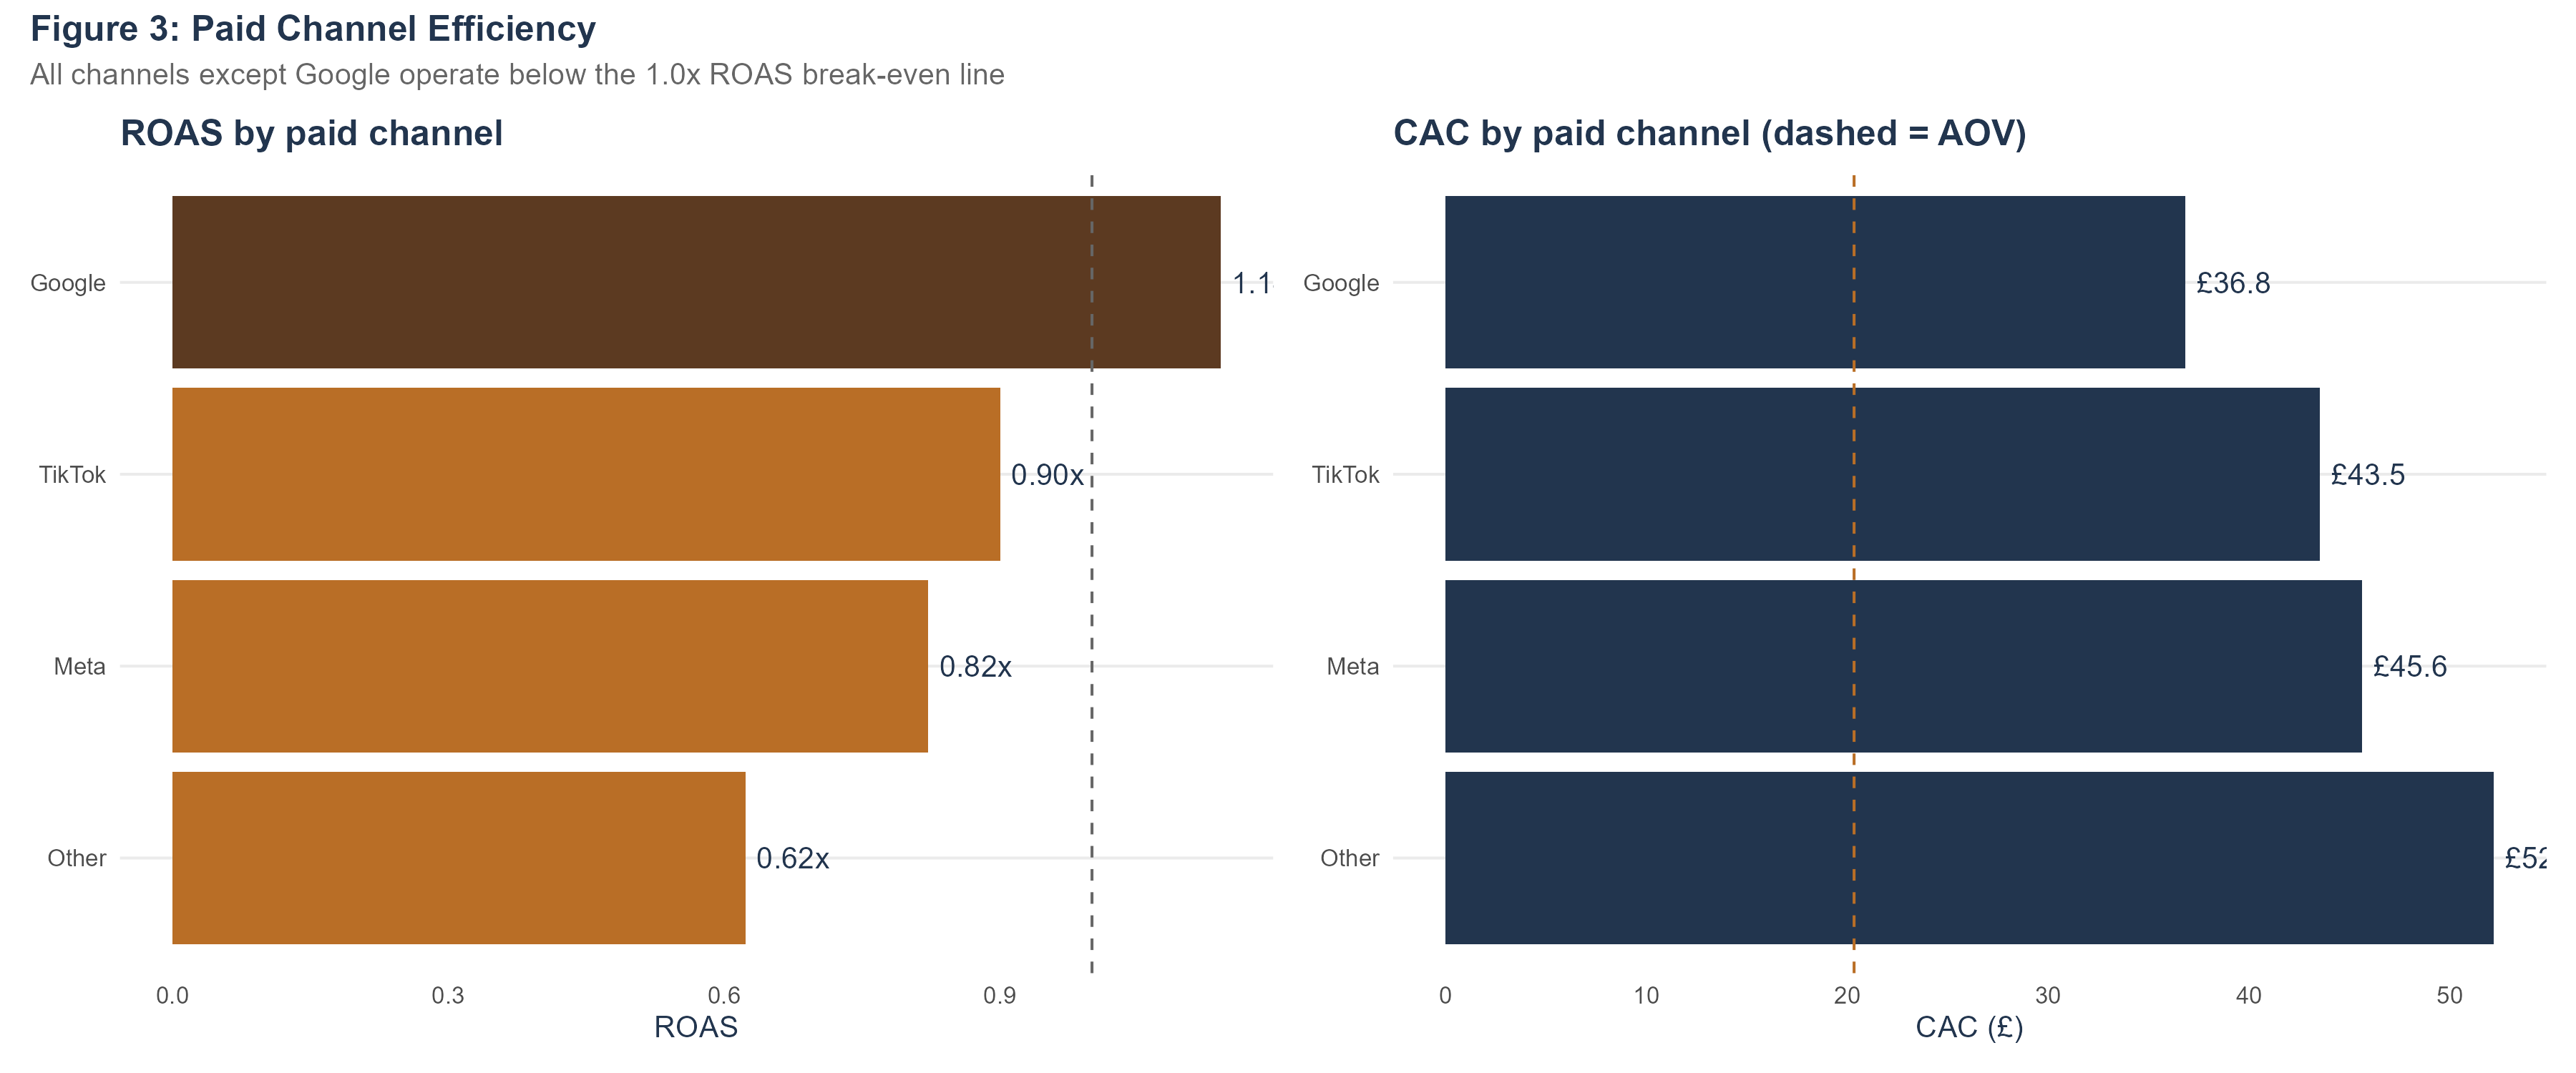
\includegraphics[width=0.95\linewidth]{figures/fig3_channel_roas_cac} 

}

\caption{Figure 3: Paid channel efficiency. Left panel — ROAS by channel against the 1.0× break-even (dashed). Right panel — CAC vs the AOV reference line (dashed copper).}\label{fig:unnamed-chunk-10}
\end{figure}

\begin{longtable}[]{@{}lrrllrll@{}}
\caption{Paid channel performance across Mar 2024 -- Feb 2026 (computed
in script 02).}\tabularnewline
\toprule\noalign{}
Channel & Spend & Clicks & CTR & CPC & Conv & ROAS & CAC \\
\midrule\noalign{}
\endfirsthead
\toprule\noalign{}
Channel & Spend & Clicks & CTR & CPC & Conv & ROAS & CAC \\
\midrule\noalign{}
\endhead
\bottomrule\noalign{}
\endlastfoot
Google & 34204 & 75830 & 4.04\% & £0.45 & 929 & 1.14× & £36.82 \\
TikTok & 12577 & 24561 & 1.81\% & £0.51 & 289 & 0.90× & £43.52 \\
Meta & 42467 & 75243 & 1.62\% & £0.56 & 931 & 0.82× & £45.61 \\
Other & 6105 & 10601 & 1.07\% & £0.58 & 117 & 0.62× & £52.18 \\
\end{longtable}

\subsubsection{Regional concentration}\label{regional-concentration}

The North East drives \textbf{20.1\% of revenue} despite being one of
eleven UK regions in the dataset (Figure 4). South East (15.4\%) and
North West (11.5\%) follow. The diversification is broad because
in-store referrals and word-of-mouth do not respect geography, but the
\emph{digital} growth thesis should still concentrate on the home
market: local SEO and click-and-collect have the lowest CAC and the
highest LTV through repeat rates.

\begin{figure}

{\centering 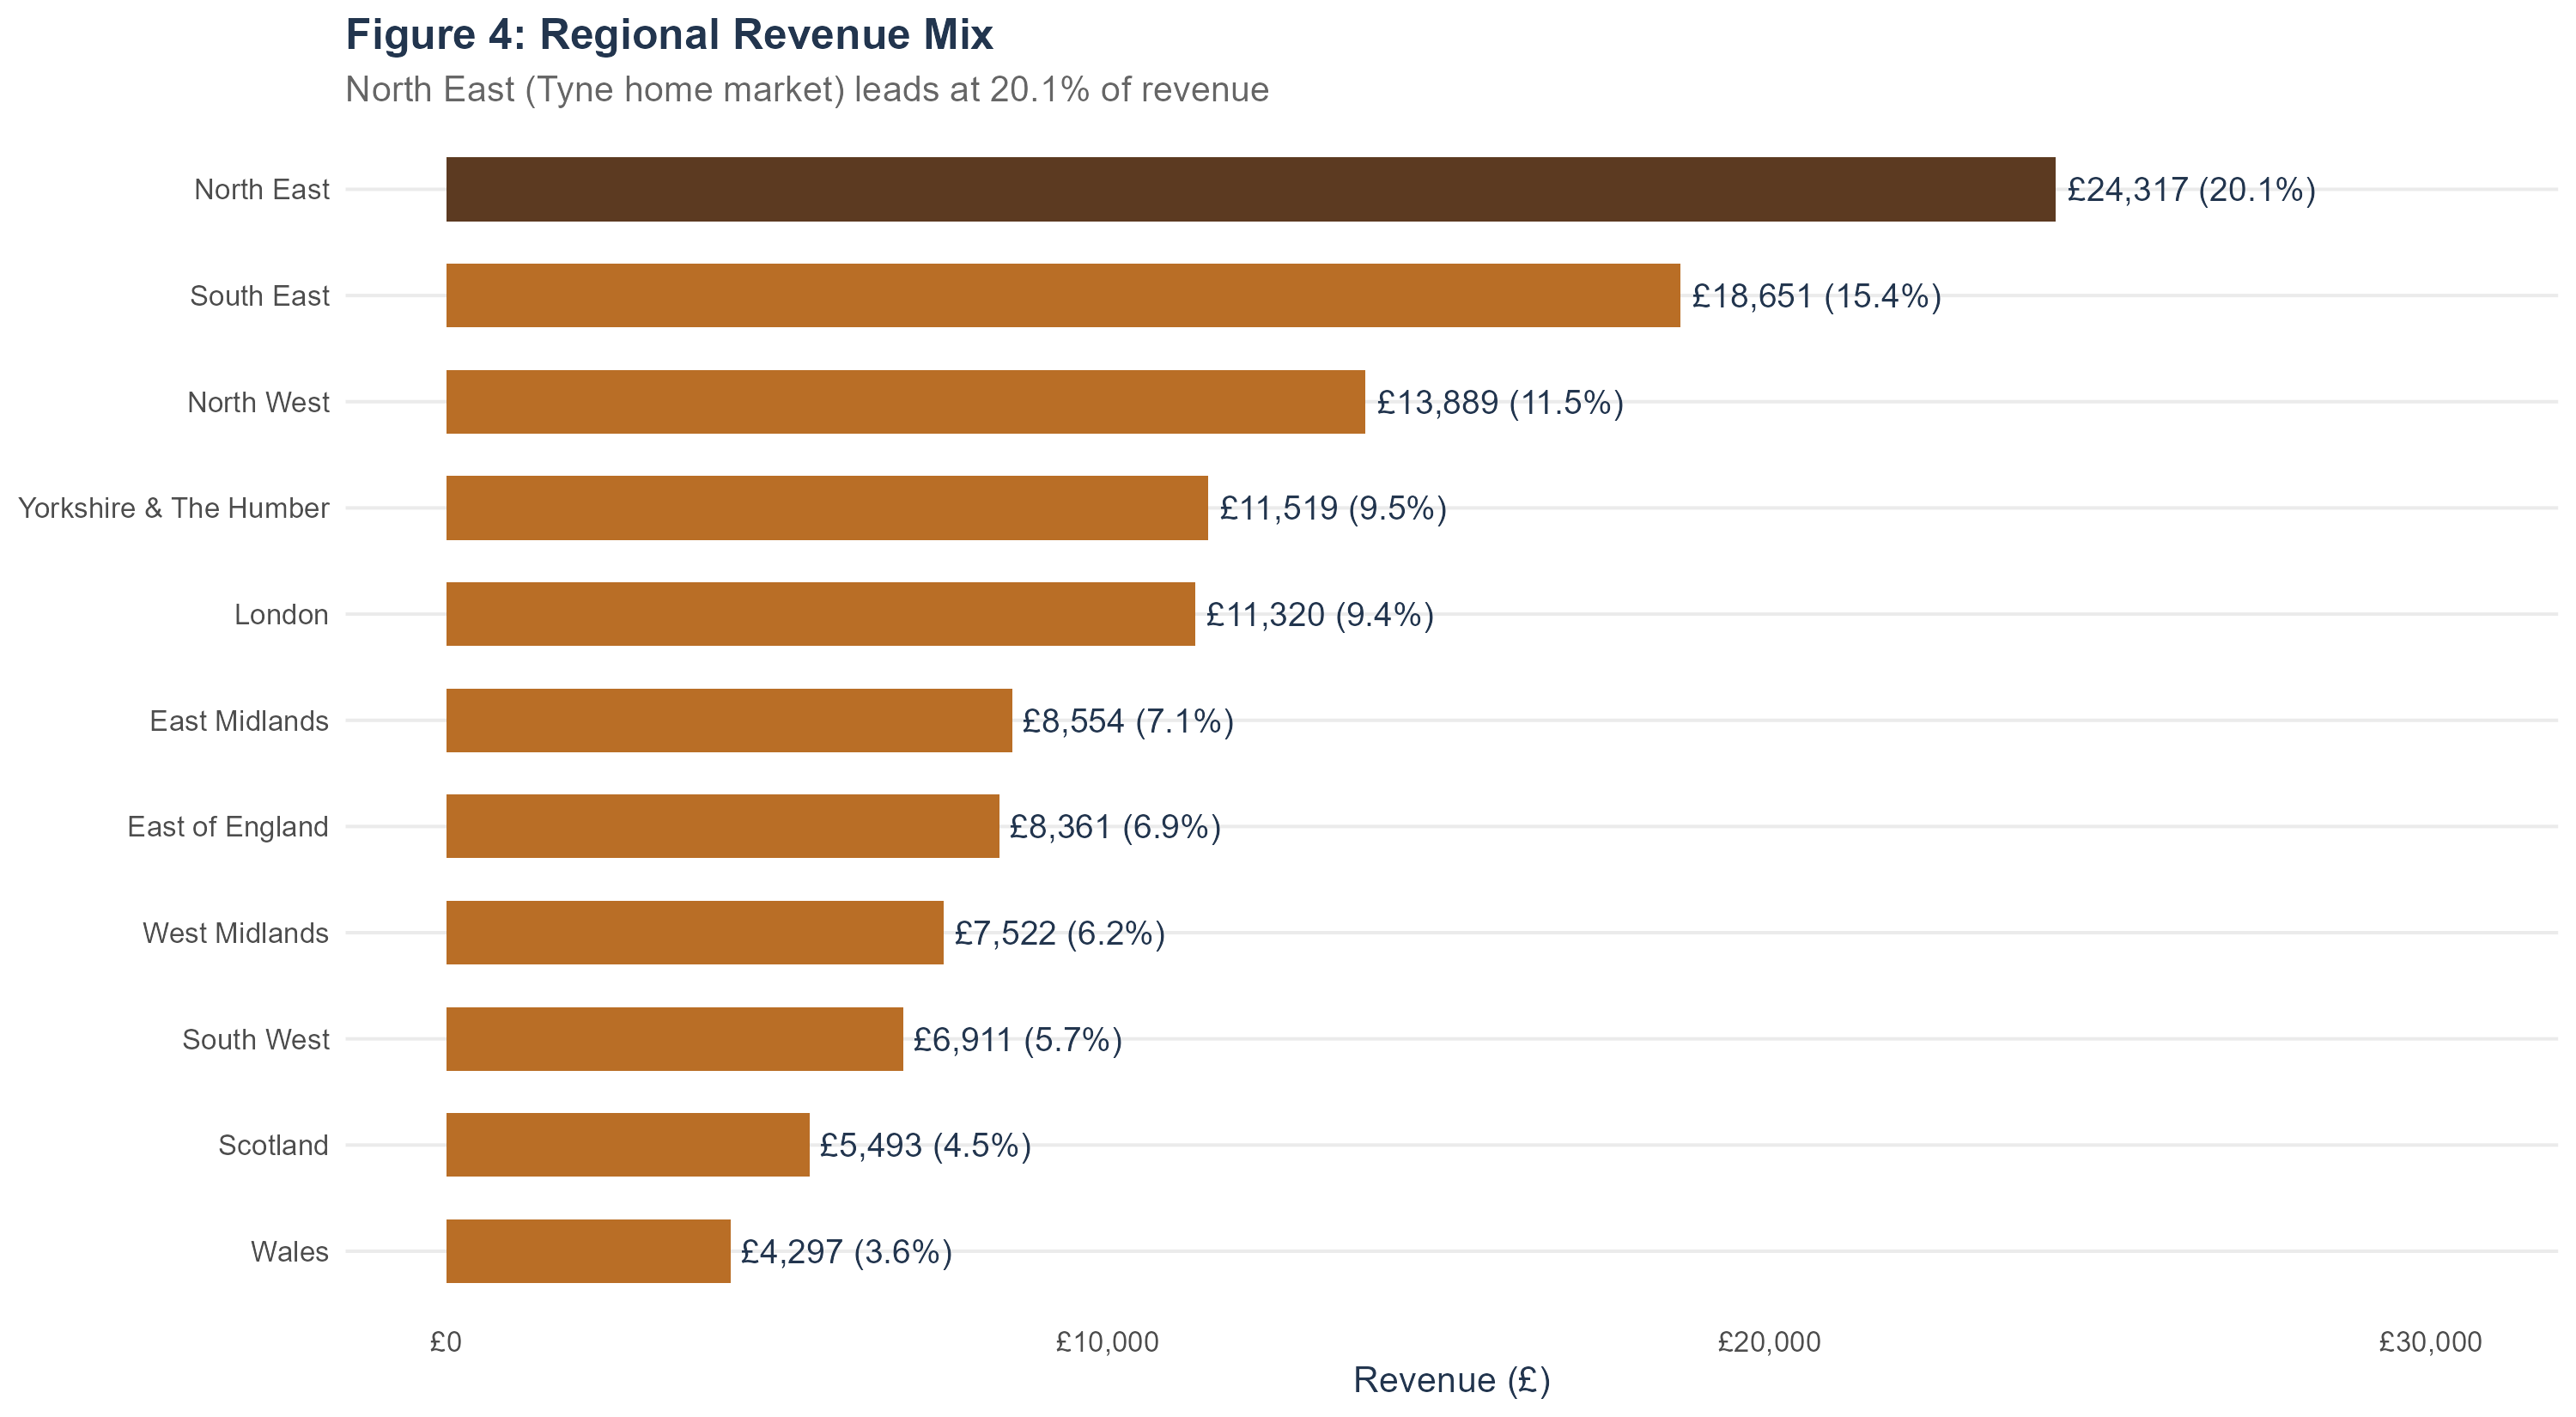
\includegraphics[width=0.95\linewidth]{figures/fig4_region_mix} 

}

\caption{Figure 4: Regional revenue mix. North East (highlighted) is the natural digital starting market.}\label{fig:unnamed-chunk-12}
\end{figure}

\subsubsection{Product and channel mix}\label{product-and-channel-mix}

Sourdough loaves account for \textbf{44\% of revenue}, with celebration
cakes (20.5\%), the subscription Bread Box (17.7\%) and pastries
(17.4\%) close behind. Mobile carries \textbf{69\% of orders} and
organic search drives \textbf{32\% of revenue} --- both reinforcing the
mobile-first, SEO-first design choices (Figure 13).

\begin{figure}

{\centering 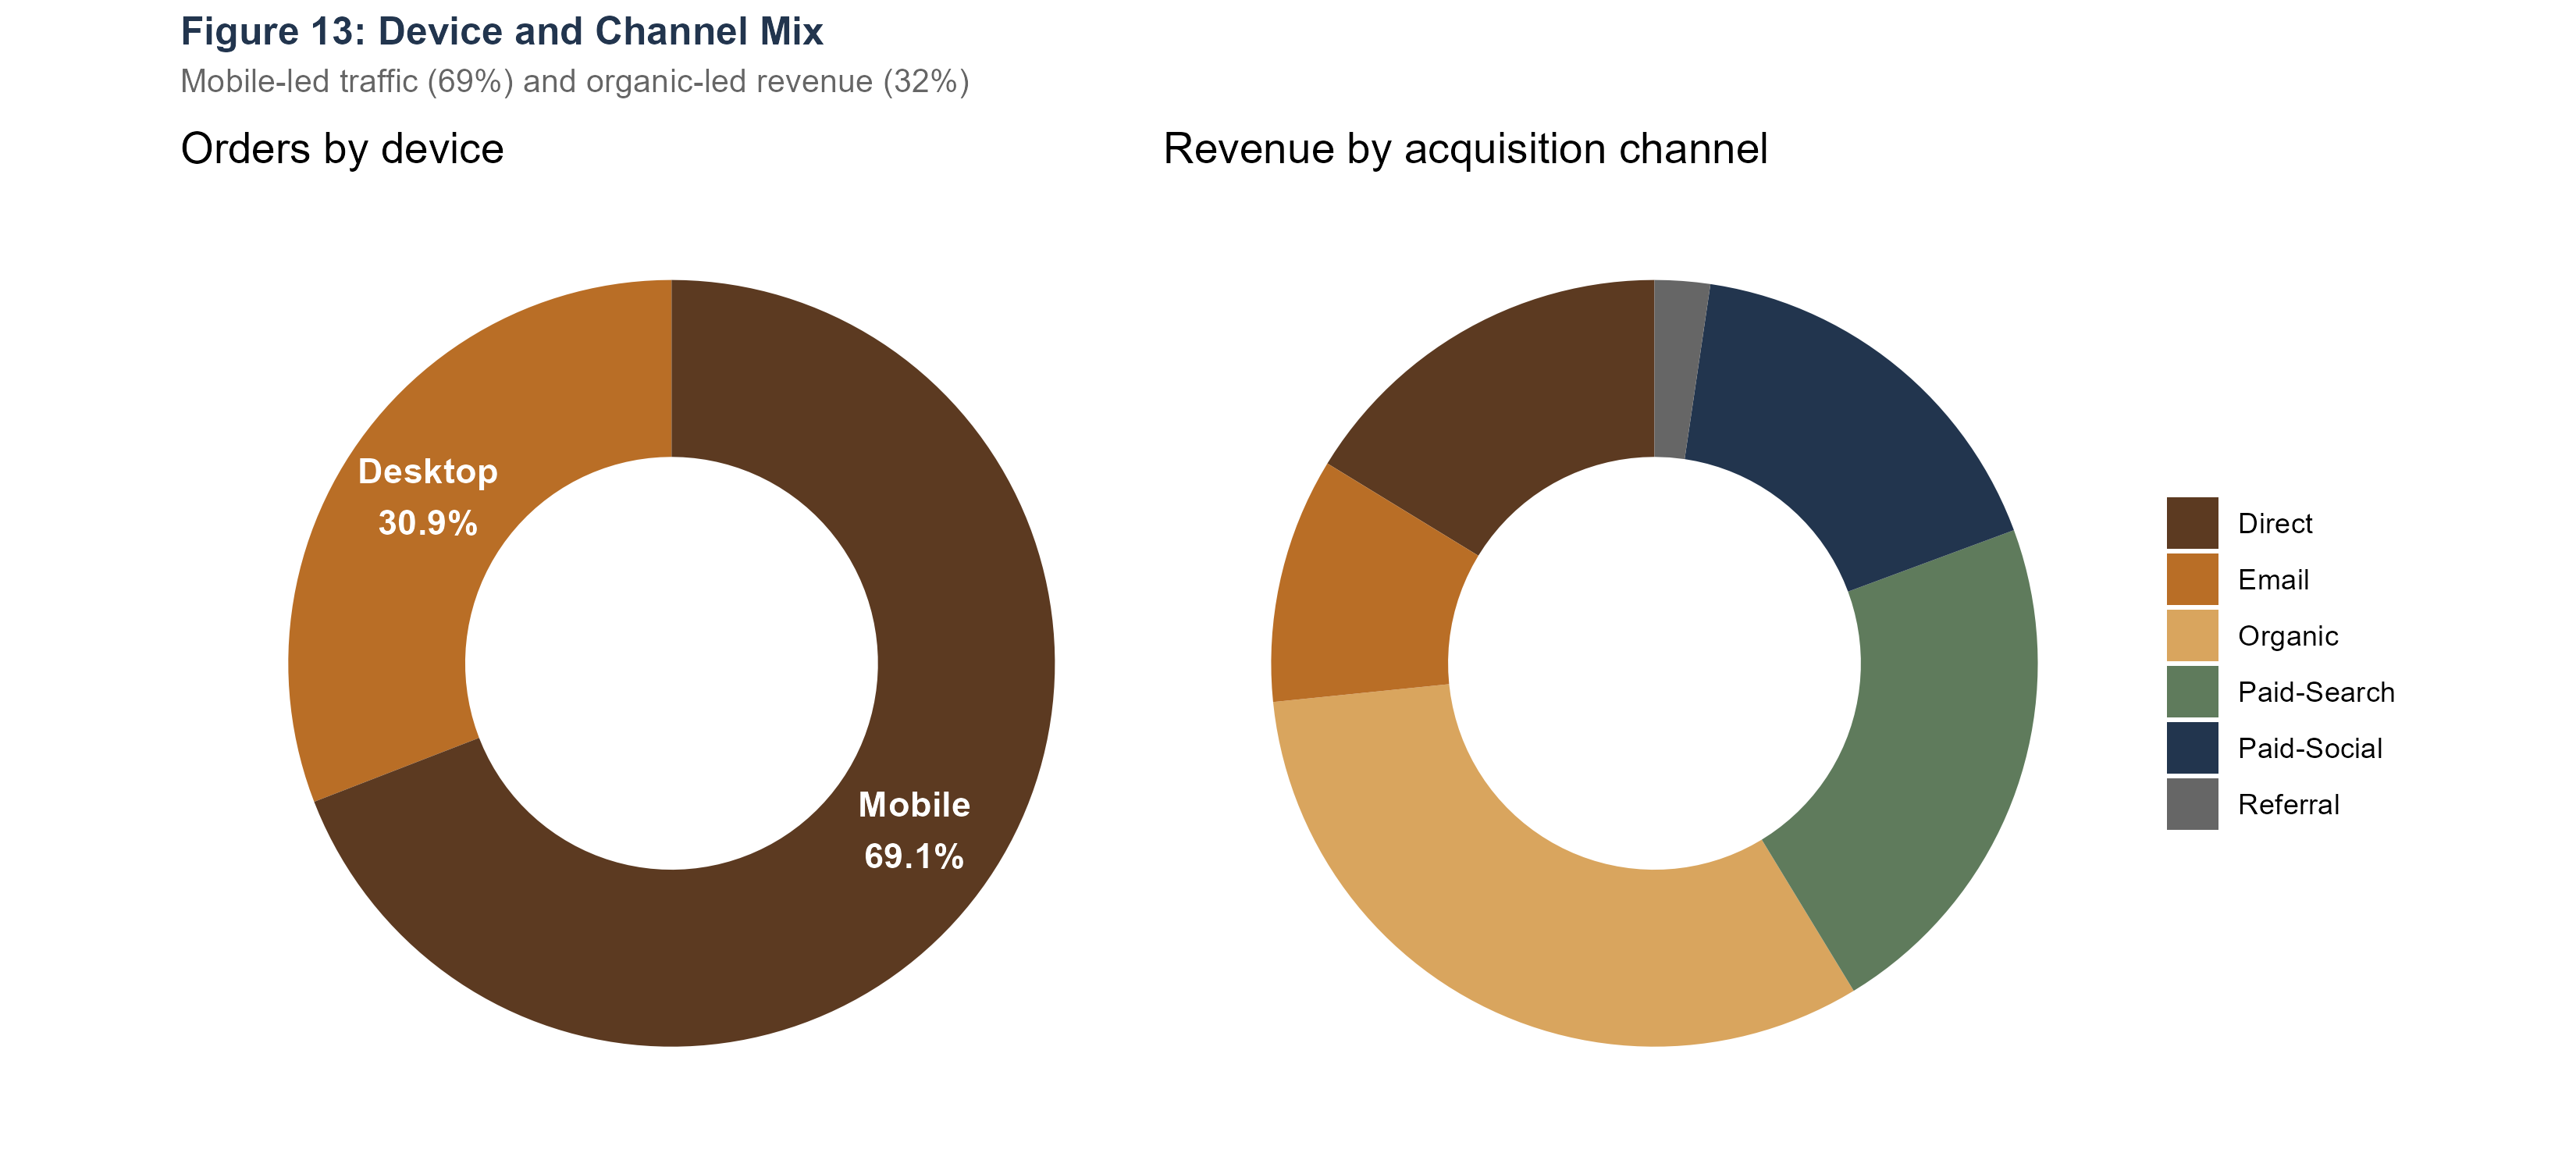
\includegraphics[width=0.95\linewidth]{figures/fig13_device_channel} 

}

\caption{Figure 13: Device and channel mix — mobile-led traffic and organic-led revenue.}\label{fig:unnamed-chunk-13}
\end{figure}

\subsubsection{Seasonality}\label{seasonality}

Contrary to the brief's expectation that \emph{Easter} would be a peak,
the data shows the \textbf{Christmas/winter window (Nov--Feb)} is the
revenue peak --- February alone delivers £18.7k, and Dec--Jan together
add a further £26.0k. Spring (Mar--Apr) is the trough. The owners should
therefore plan an \textbf{aggressive Christmas campaign} with 6--8 week
lead-in and a reduced spring tempo (Figure 11).

\begin{figure}

{\centering 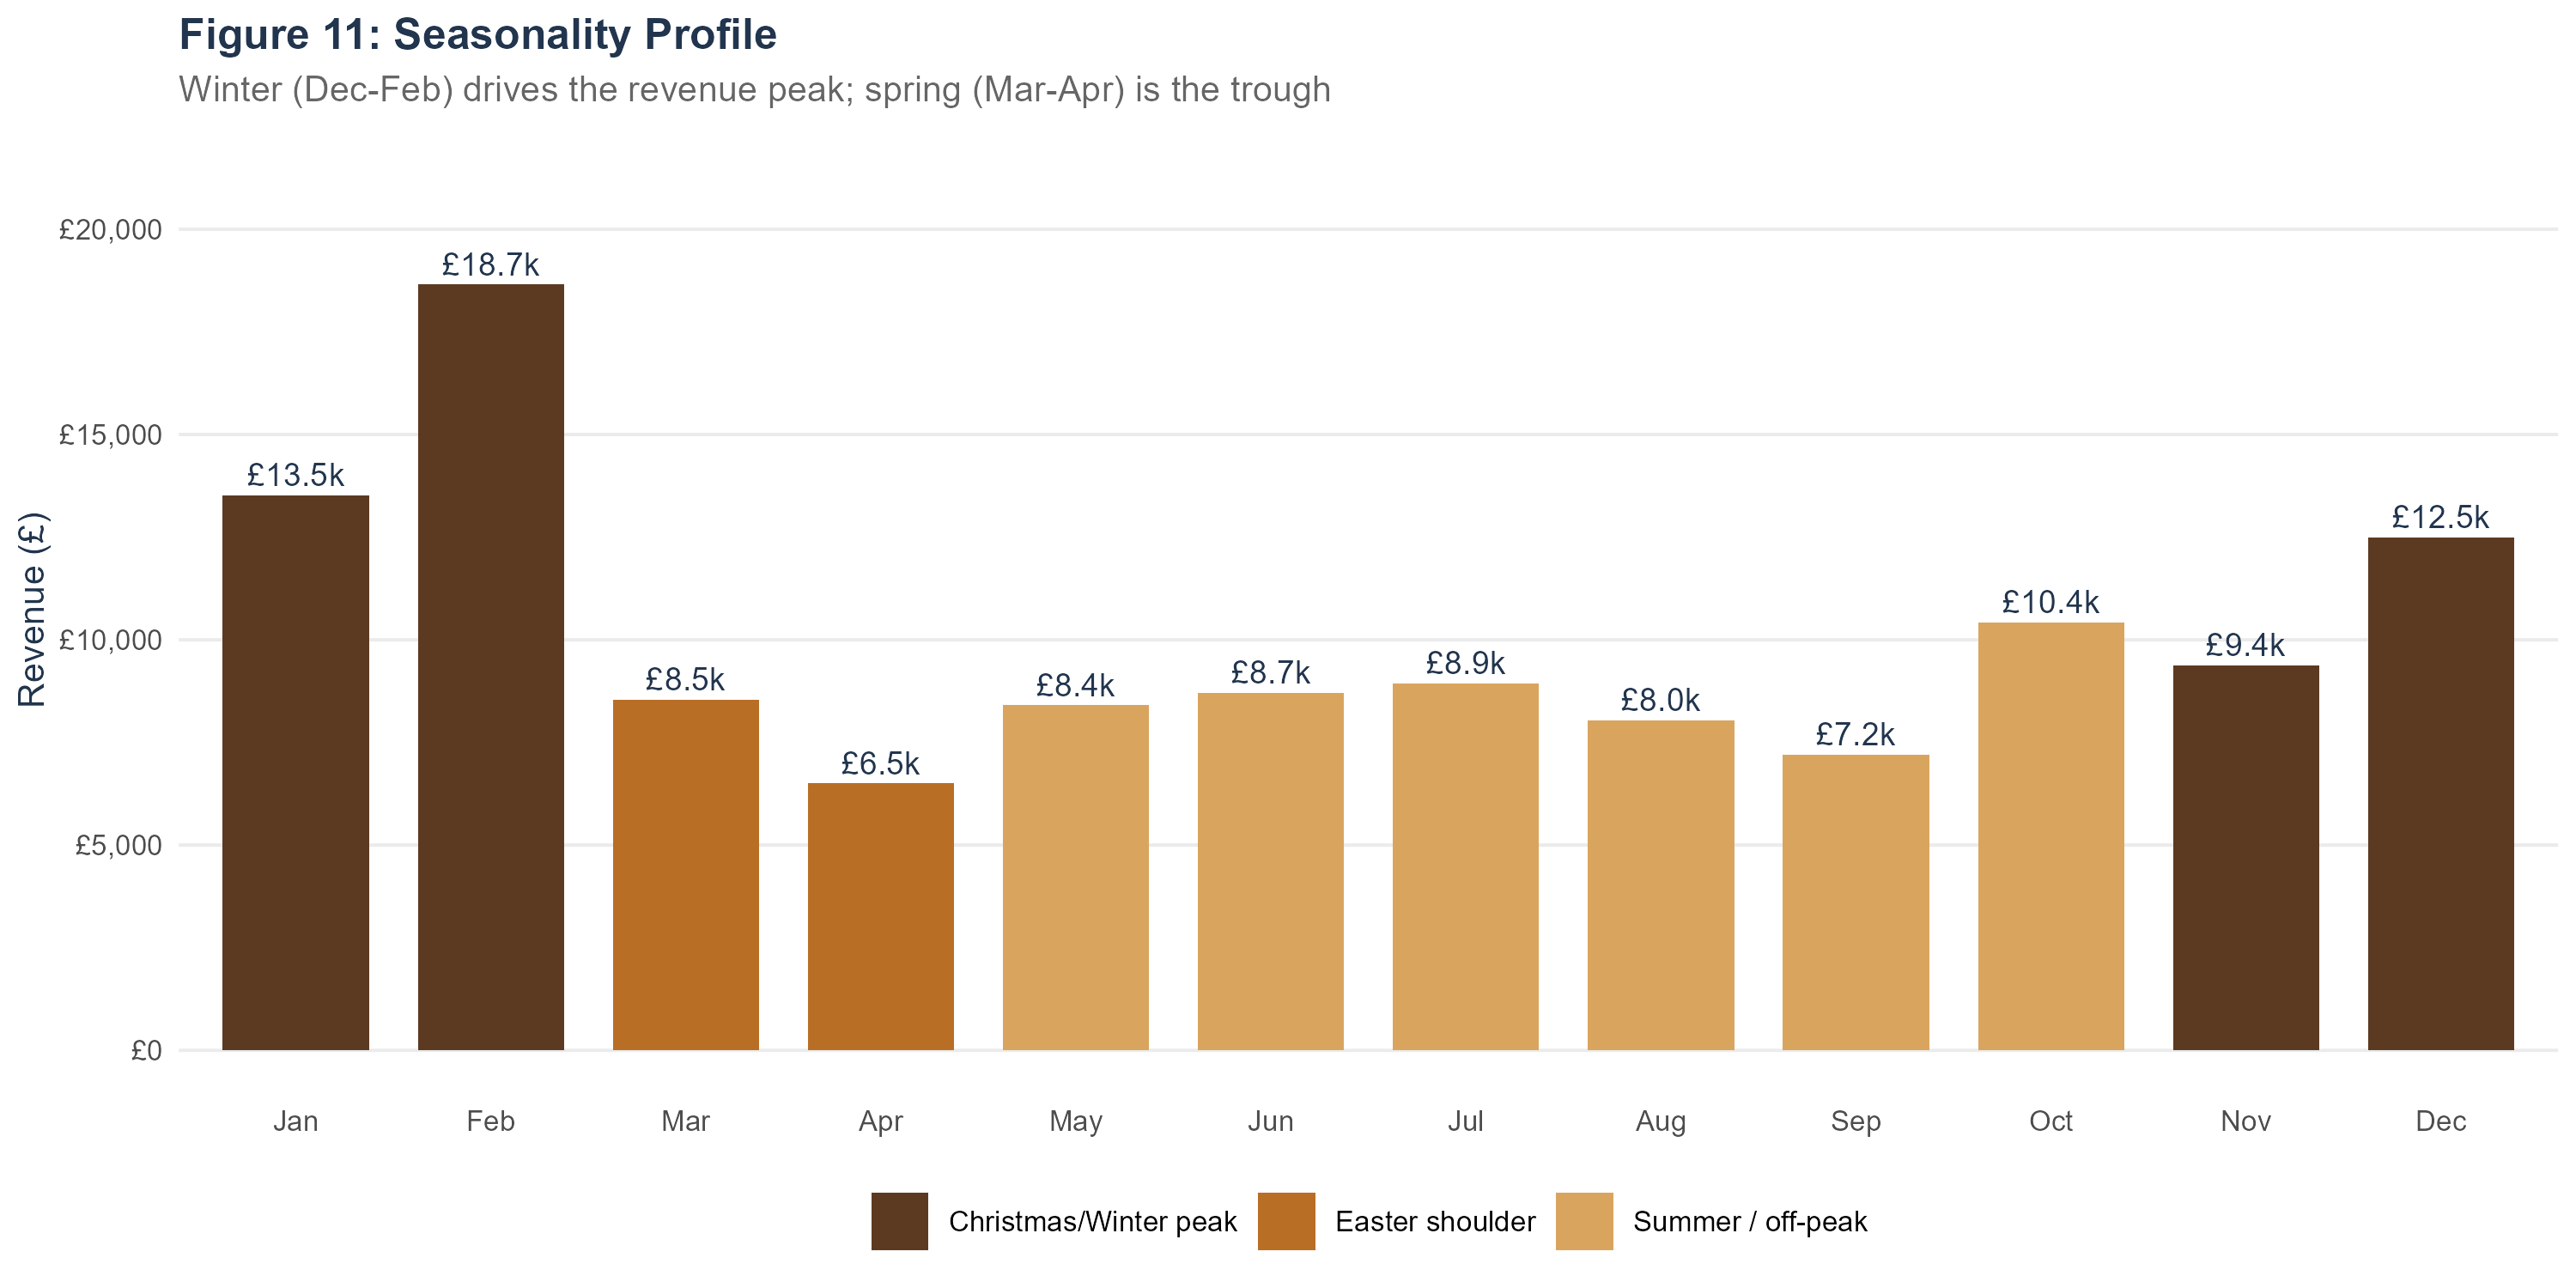
\includegraphics[width=0.95\linewidth]{figures/fig11_seasonality} 

}

\caption{Figure 11: Month-of-year seasonality. Brown = Christmas/Winter peak; copper = Easter shoulder; wheat = summer/off-peak.}\label{fig:unnamed-chunk-14}
\end{figure}

\subsubsection{Subscription dynamics and
churn}\label{subscription-dynamics-and-churn}

Active subscriptions grew from \textasciitilde110 in mid-2024 to
\textasciitilde560 by February 2026, with \textbf{average monthly churn
of 4.5\%} (Figure 12). Subscription share of orders has \emph{fallen}
from a 2024 peak of 26\% to \textasciitilde14\% in early 2026, because
new acquisition has outpaced subscription conversion --- a known
phenomenon in DTC food (Recharge, 2024). The plan addresses this through
the AI recommendation engine and a Q4 loyalty/subscription gifting
campaign.

\begin{figure}

{\centering 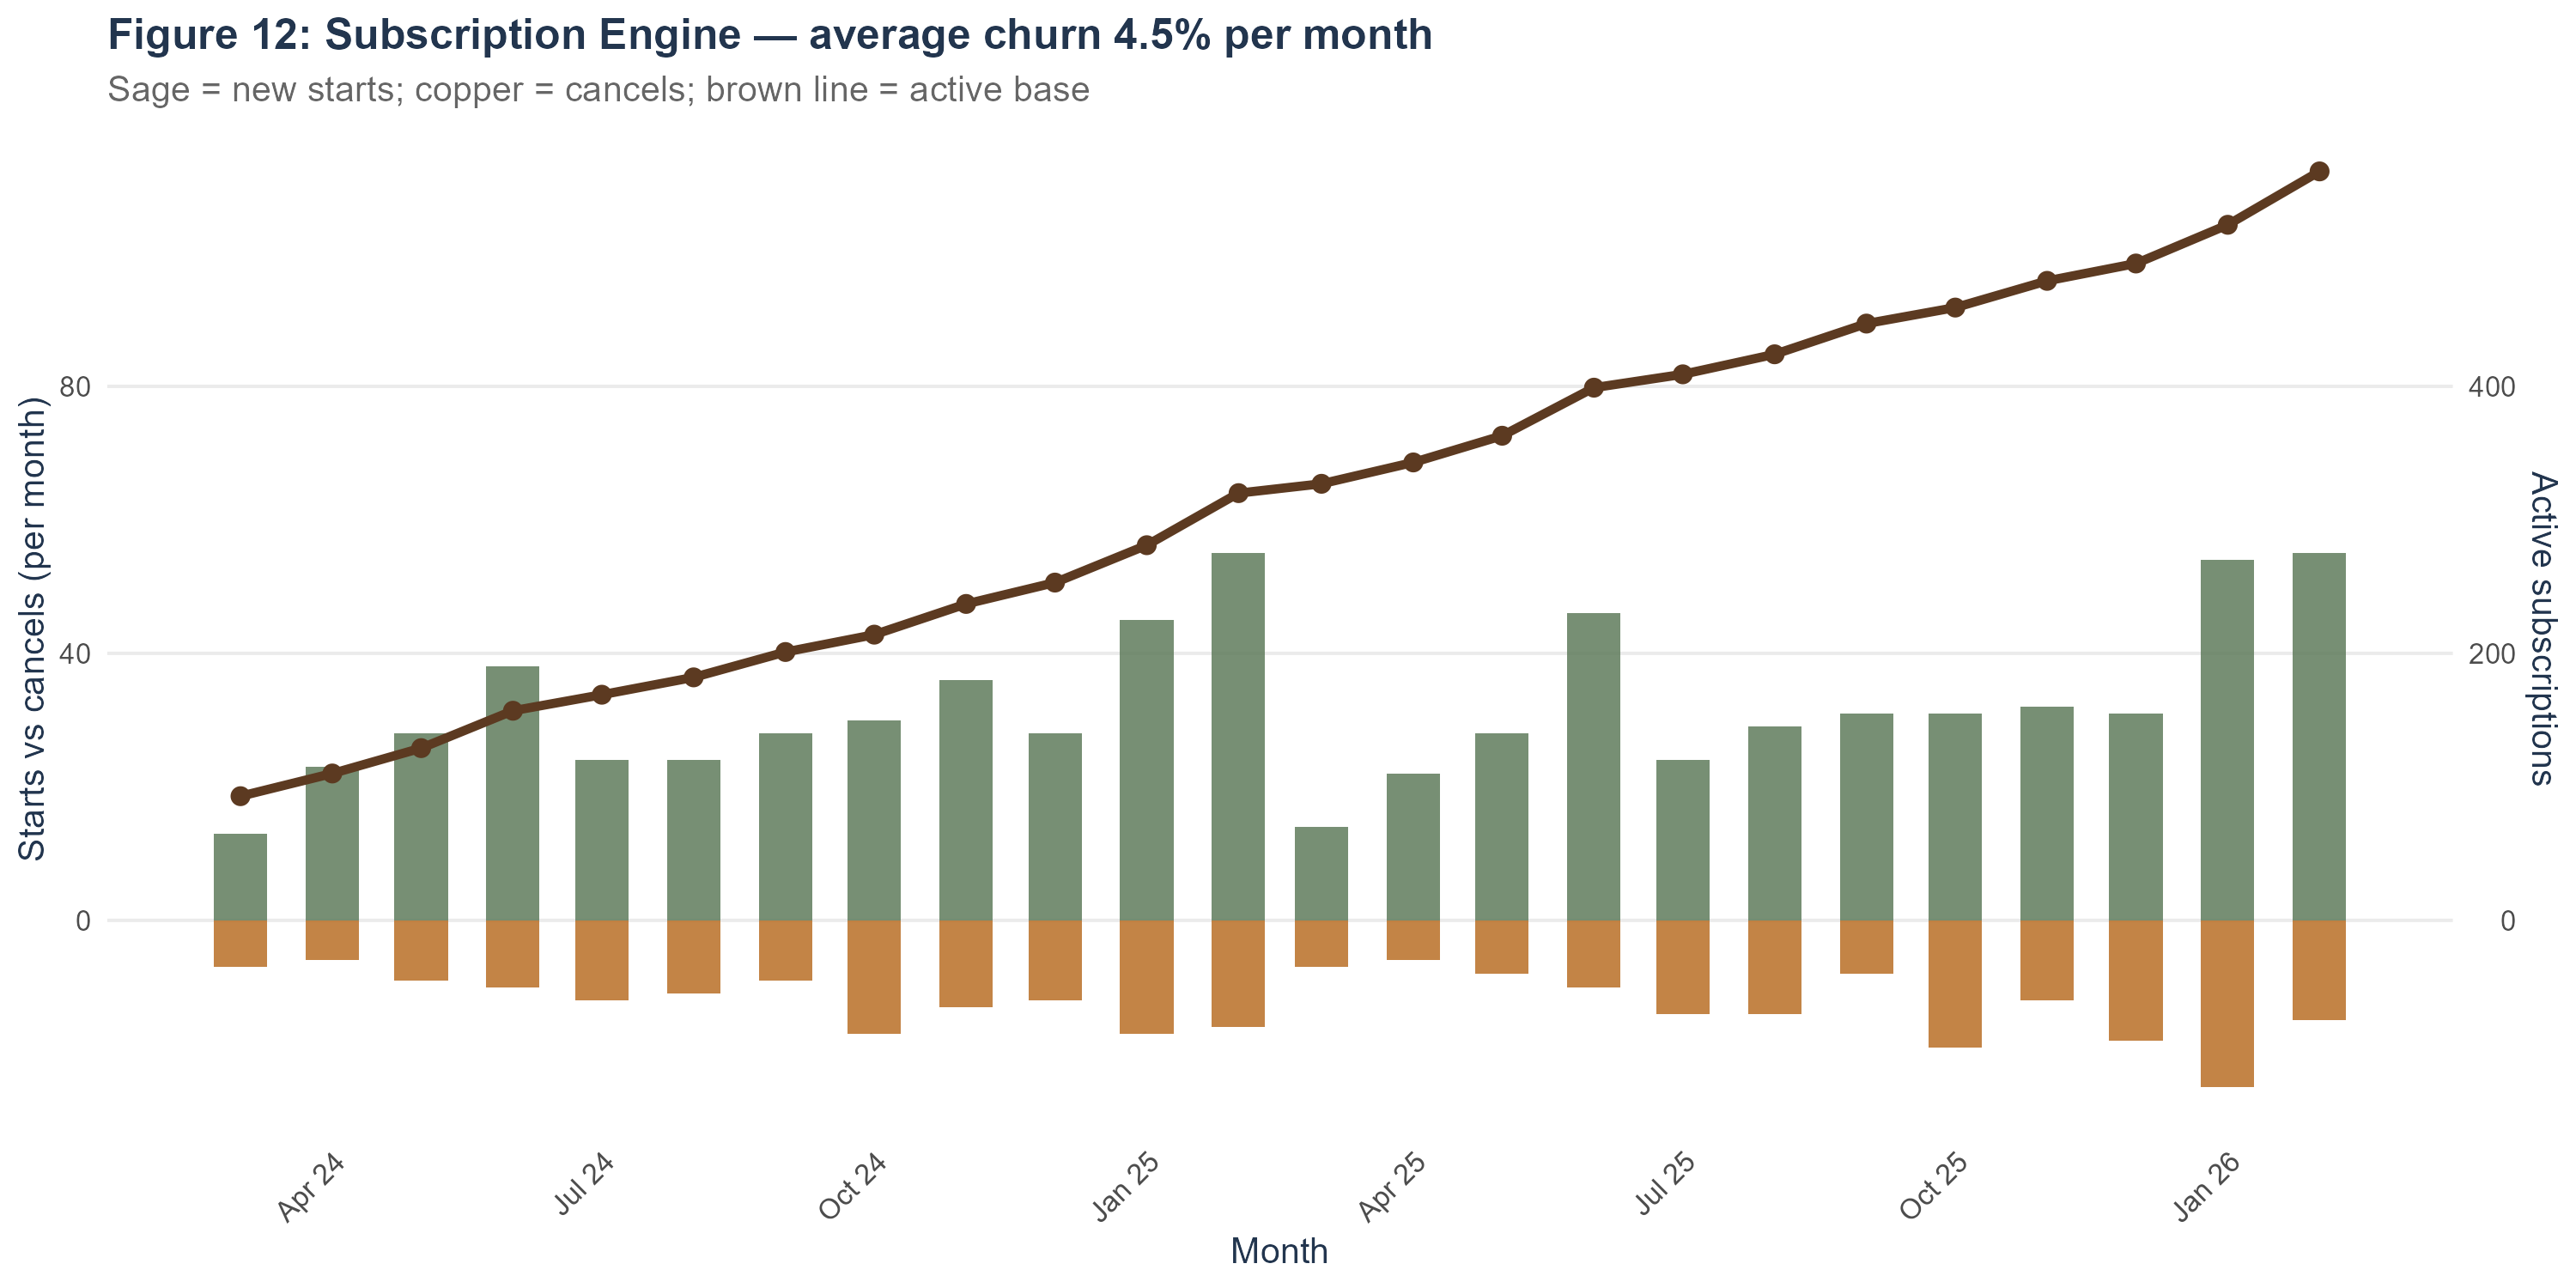
\includegraphics[width=0.95\linewidth]{figures/fig12_subscription_dynamics} 

}

\caption{Figure 12: Subscription dynamics. Sage bars = new starts; copper bars (below zero) = cancels; brown line = active subscription base.}\label{fig:unnamed-chunk-15}
\end{figure}

\subsubsection{A/B test outcome}\label{ab-test-outcome}

Variant B (image-led hero with subscription cross-sell) converted at
\textbf{3.65\%} versus Variant A control at \textbf{2.86\%} on 96,700
visitors --- a \textbf{+27.5\% relative uplift} with a two-proportion
z-statistic of 6.90 (p \textless{} 0.001). The 95\% confidence intervals
do not overlap (Figure 5), and the effect is more than double the
pre-registered MDE; we recommend \textbf{immediate roll-out}.

\begin{figure}

{\centering 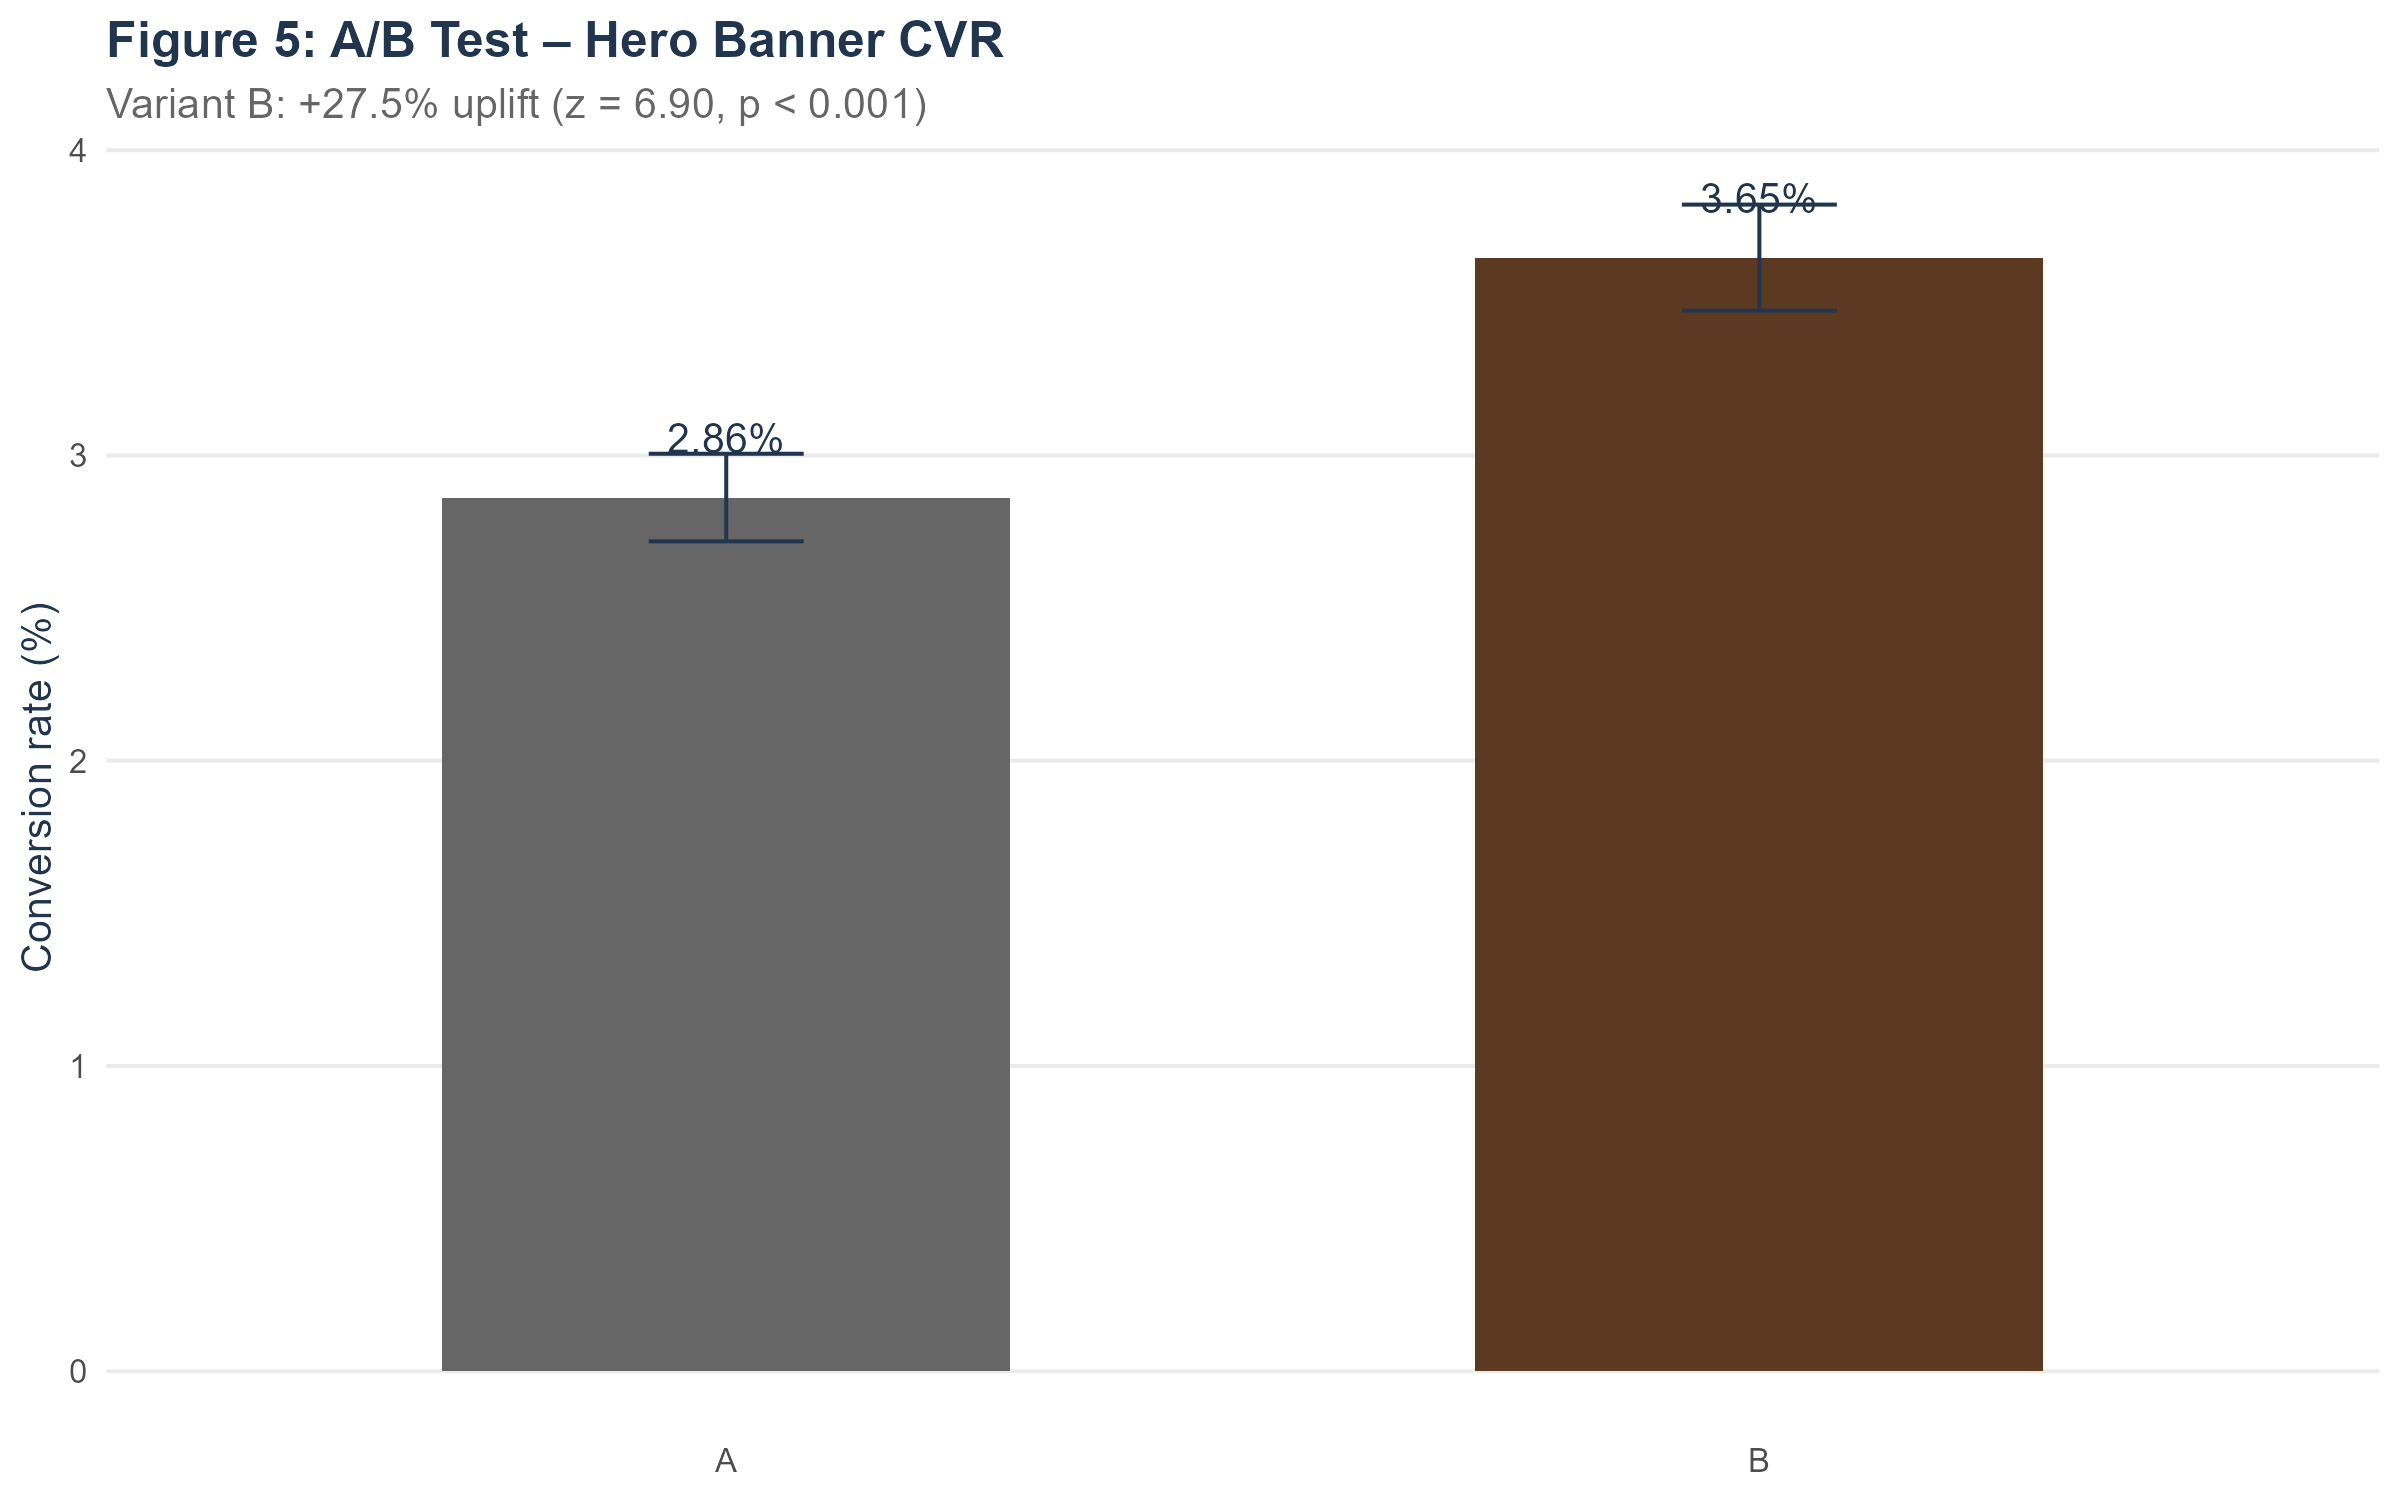
\includegraphics[width=0.95\linewidth]{figures/fig5_ab_test_uplift} 

}

\caption{Figure 5: A/B test result with 95\% confidence intervals. Variant B's uplift is highly statistically significant (z = 6.90, p < 0.001).}\label{fig:unnamed-chunk-16}
\end{figure}

\subsection{Forecast, Budget Reallocation and
Roadmap}\label{forecast-budget-reallocation-and-roadmap}

\subsubsection{Triangulated assumptions}\label{triangulated-assumptions}

The Base scenario assumes a \textbf{4\% monthly compound MALC growth}
because it matches (i) the trailing-12-month observed CAGR, (ii) UK SME
e-commerce benchmarks for new-launch DTC food (Statista, 2025), and
(iii) bottom-up unit economics (organic AOV × email-driven repeat-rate).
Low and High scenarios capture ±2pp parameter uncertainty.

\subsubsection{12-month forecast}\label{month-forecast}

\begin{figure}

{\centering 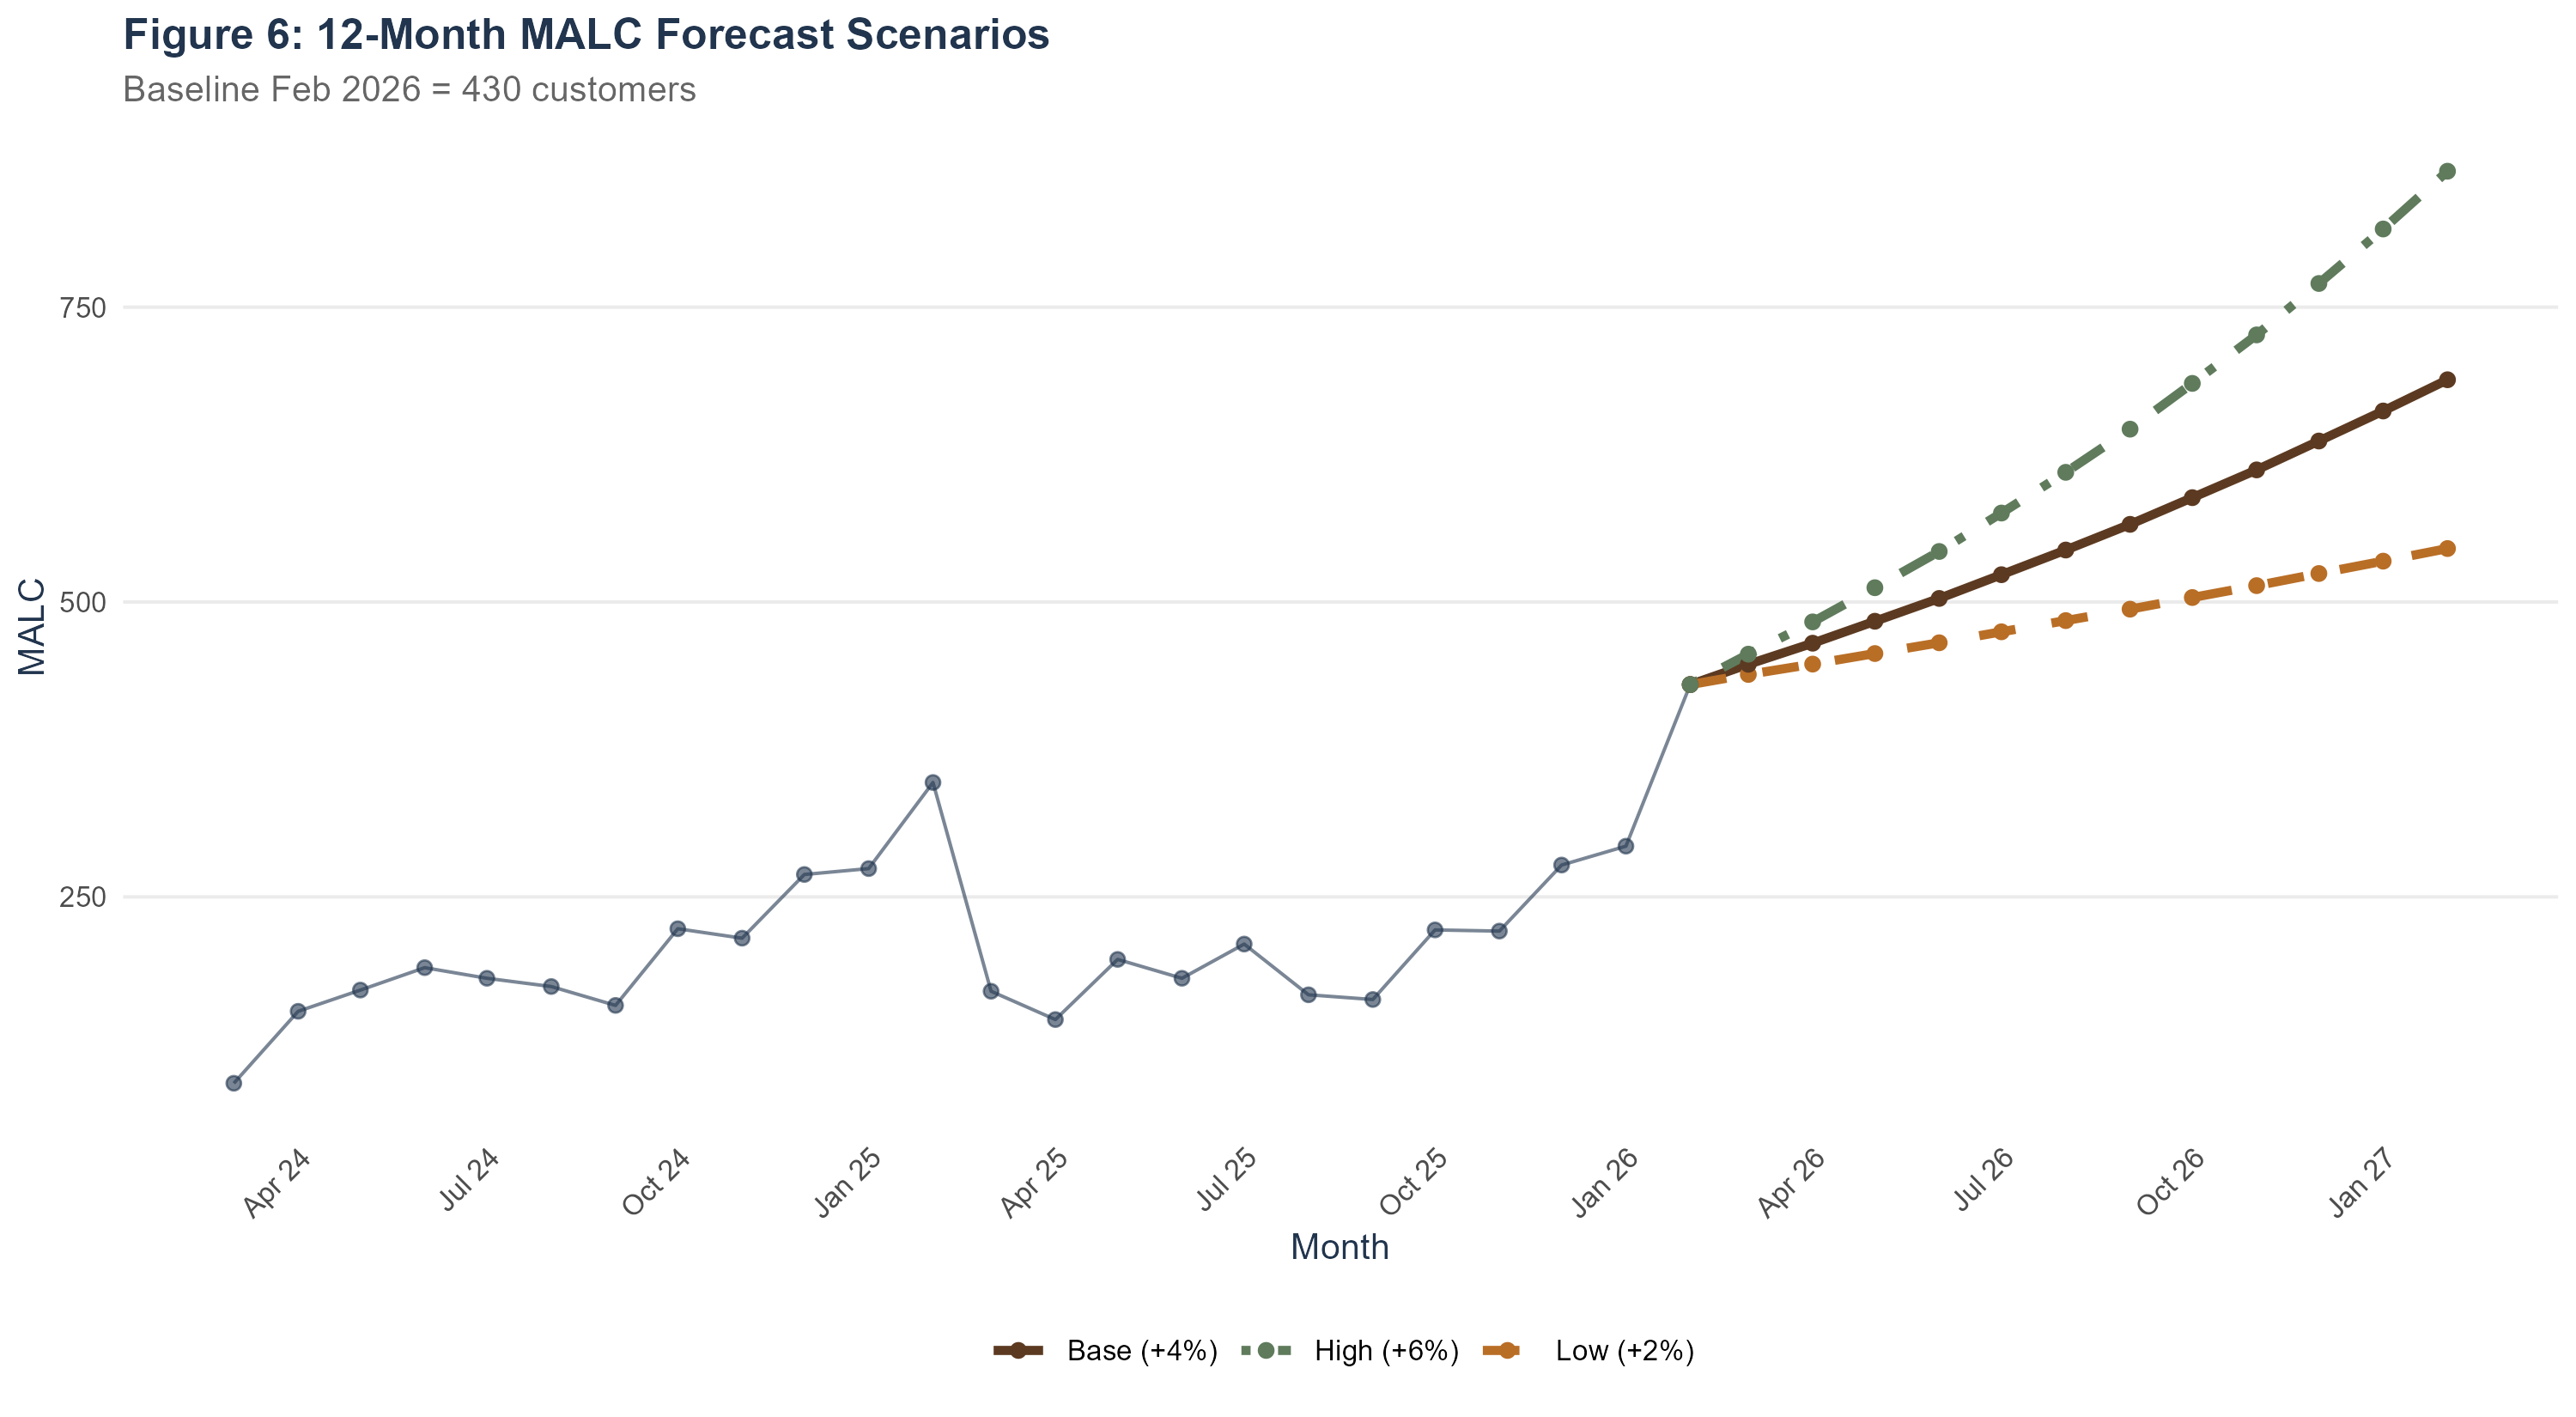
\includegraphics[width=0.95\linewidth]{figures/fig6_forecast_scenarios} 

}

\caption{Figure 6: Twelve-month MALC forecast under Low (+2\% mo), Base (+4\% mo) and High (+6\% mo) scenarios. Baseline = 430 MALC at February 2026.}\label{fig:unnamed-chunk-17}
\end{figure}

\begin{longtable}[]{@{}lllllll@{}}
\caption{Forecast outputs by scenario. MALC values are integer
customers; revenue is computed at AOV £20.34.}\tabularnewline
\toprule\noalign{}
Scenario & M+3 & M+6 & M+9 & M+12 & Revenue M+12 (£) & Δ vs baseline \\
\midrule\noalign{}
\endfirsthead
\toprule\noalign{}
Scenario & M+3 & M+6 & M+9 & M+12 & Revenue M+12 (£) & Δ vs baseline \\
\midrule\noalign{}
\endhead
\bottomrule\noalign{}
\endlastfoot
Low (+2\%/mo) & 456 & 484 & 513 & 545 & 11,094 & +27\% \\
Base (+4\%/mo) & 484 & 544 & 612 & 688 & 14,008 & +60\% \\
High (+6\%/mo) & 512 & 610 & 726 & 865 & 17,615 & +101\% \\
\end{longtable}

\subsubsection{Budget reallocation}\label{budget-reallocation}

Applying a ROAS-rank reallocation rule (Top-1 × 1.30, Top-2 × 1.05,
Top-3 × 0.85, bottom × 0.55) to the Mar-24 -- Feb-26 paid history yields
the shift in Figure 15: \textbf{Google +15 pp}, \textbf{TikTok and Meta
cut}, \textbf{Other heavily reduced}. This is the policy that will be
re-run at the end of each quarter.

\begin{figure}

{\centering 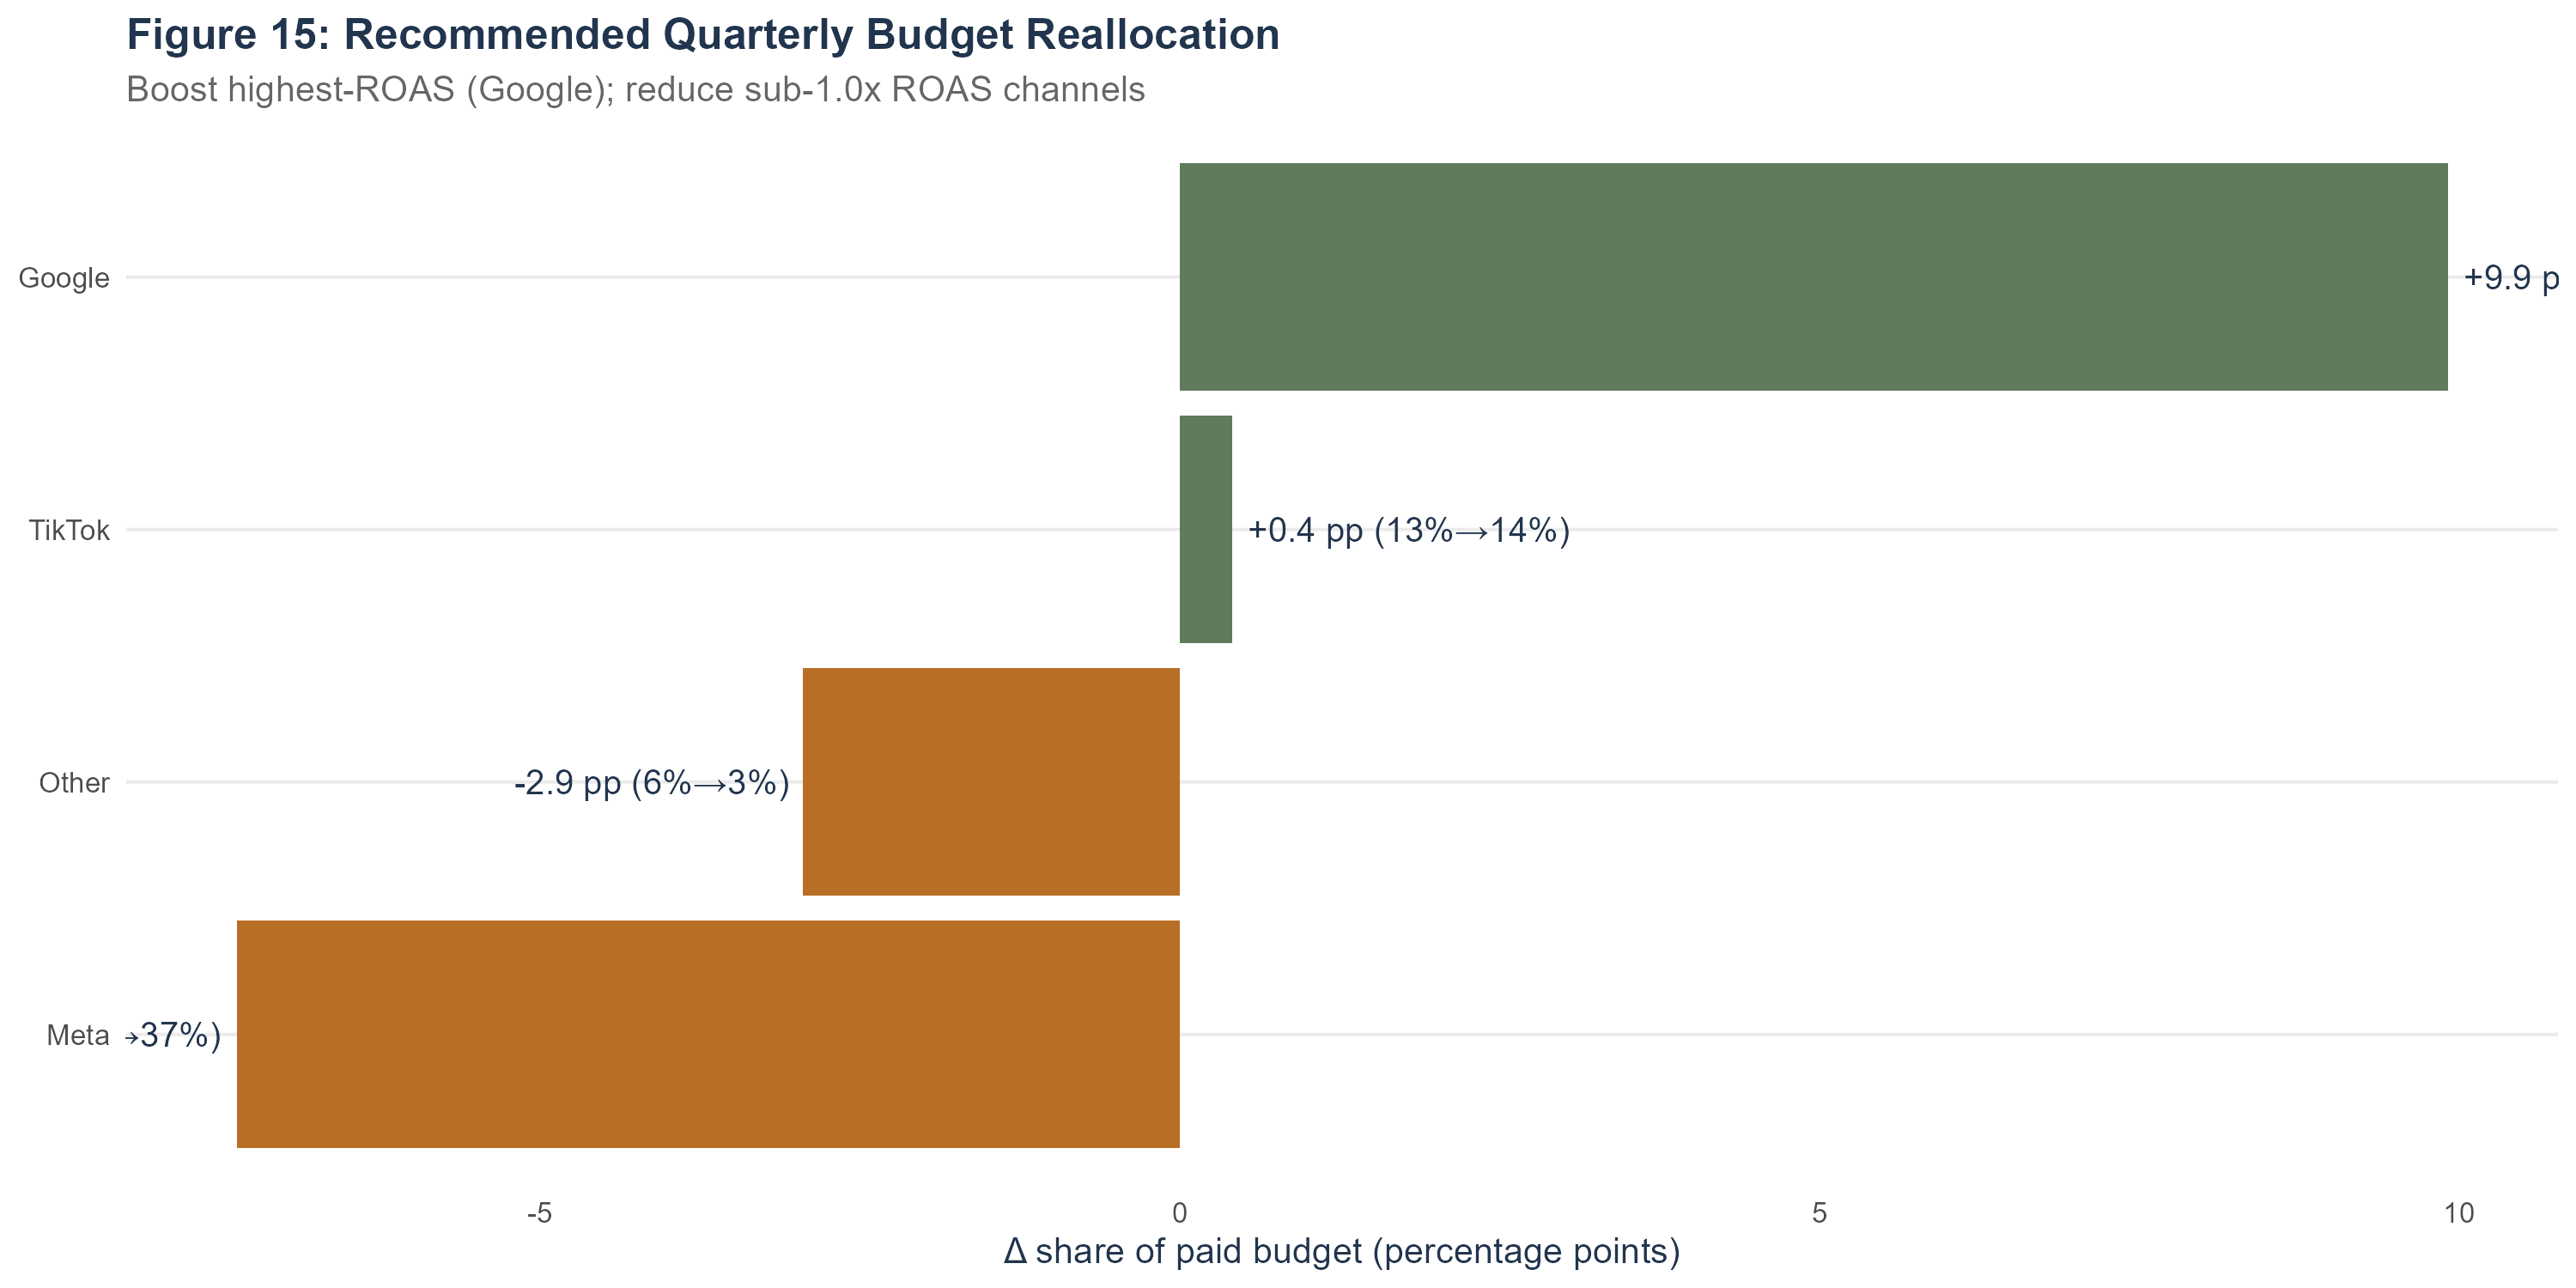
\includegraphics[width=0.95\linewidth]{figures/fig15_budget_reallocation} 

}

\caption{Figure 15: Recommended quarterly budget reallocation. Sage = increase, copper = decrease. The single highest-ROAS channel (Google) gains share at the expense of sub-1.0× ROAS channels.}\label{fig:unnamed-chunk-19}
\end{figure}

\subsubsection{Retention and CLV
consideration}\label{retention-and-clv-consideration}

A simplified Pareto/NBD-lite CLV (Fader, Hardie \& Lee, 2005) yields a
12-month CLV of approximately \textbf{£55} per active customer at the
current 4.5\% churn and 55\% gross margin. Reducing churn by 1 pp (to
3.5\%) lifts CLV by \textasciitilde29\% --- which is why the retention
investments in Q3 / Q4 are part of the plan rather than an afterthought.

\subsubsection{Quarterly roadmap}\label{quarterly-roadmap}

\begin{longtable}[]{@{}
  >{\raggedright\arraybackslash}p{(\linewidth - 6\tabcolsep) * \real{0.0842}}
  >{\raggedright\arraybackslash}p{(\linewidth - 6\tabcolsep) * \real{0.7158}}
  >{\raggedright\arraybackslash}p{(\linewidth - 6\tabcolsep) * \real{0.1263}}
  >{\raggedright\arraybackslash}p{(\linewidth - 6\tabcolsep) * \real{0.0737}}@{}}
\caption{Quarterly roadmap with expected MALC uplift and indicative
budget.}\tabularnewline
\toprule\noalign{}
\begin{minipage}[b]{\linewidth}\raggedright
Quarter
\end{minipage} & \begin{minipage}[b]{\linewidth}\raggedright
Focus
\end{minipage} & \begin{minipage}[b]{\linewidth}\raggedright
MALC uplift
\end{minipage} & \begin{minipage}[b]{\linewidth}\raggedright
Budget
\end{minipage} \\
\midrule\noalign{}
\endfirsthead
\toprule\noalign{}
\begin{minipage}[b]{\linewidth}\raggedright
Quarter
\end{minipage} & \begin{minipage}[b]{\linewidth}\raggedright
Focus
\end{minipage} & \begin{minipage}[b]{\linewidth}\raggedright
MALC uplift
\end{minipage} & \begin{minipage}[b]{\linewidth}\raggedright
Budget
\end{minipage} \\
\midrule\noalign{}
\endhead
\bottomrule\noalign{}
\endlastfoot
Q1 & Shopify MVP launch, GA4 + Klaviyo wiring, email capture, A/B winner
& +5--8\% & £2,000 \\
Q2 & SEO/blog programme; Bread Box LP; subscription gifting test &
+8--12\% & £2,500 \\
Q3 & Budget reallocation by ROAS; PDP optimisation; retention flows &
+10--15\% & £3,000 \\
Q4 & Christmas campaign; loyalty tier; subscription gifting; review &
+15--20\% & £4,000 \\
\end{longtable}

\subsection{Ethics, Privacy \&
Accessibility}\label{ethics-privacy-accessibility}

\subsubsection{GDPR-by-default}\label{gdpr-by-default}

Cookie consent uses an opt-in banner (OneTrust or Shopify Customer
Privacy API) that distinguishes strictly-necessary, analytics and
marketing cookies (ICO, 2024). All email signups use \textbf{double
opt-in} through Klaviyo, with a one-click unsubscribe in every send. A
Data Subject Access Request (DSAR) workflow is documented in Appendix B
and handled within the 30-day statutory window. Personal data is
minimised (email, name, address, phone) and retained for 24 months
post-purchase.

\subsubsection{Accessibility (WCAG 2.2
AA)}\label{accessibility-wcag-2.2-aa}

The site targets WCAG 2.2 AA (W3C, 2023). The brand palette already
meets a 4.5:1 contrast ratio. AI-generated ALT text is human-reviewed;
keyboard navigation is tested at every release; the body type is 16px
minimum with a 1.5× line-height. A monthly Axe/WAVE audit is scheduled
and an annual screen-reader walkthrough is conducted with NVDA.

\subsubsection{Responsible AI}\label{responsible-ai}

The AI layer is constrained to \emph{non-decisioning} tasks --- content
drafts and recommendations --- with founder review before send/publish.
Customer-facing AI features (e.g.~WhatsApp assistant) are disclosed in
plain English at the point of interaction, per the EU AI Act
transparency obligations (European Commission, 2024).

\newpage

\section{Recommendations and
Conclusion}\label{recommendations-and-conclusion}

\subsection{Five actionable
recommendations}\label{five-actionable-recommendations}

\begin{enumerate}
\def\labelenumi{\arabic{enumi}.}
\tightlist
\item
  \textbf{Adopt MALC as the North Star and instrument it in Week 1.}
  Every decision in the next 12 months runs off this number; without it,
  the plan reverts to bets.
\item
  \textbf{Ship the AI-augmented Shopify MVP in eight weeks}, with the
  Variant B hero in production from day one (+27.5\% CVR uplift, p
  \textless{} 0.001).
\item
  \textbf{Reverse the conventional paid split: 60\% Google, 25\% Meta,
  15\% TikTok} until Meta and TikTok ROAS clears 1.0×. Reallocate
  quarterly using the rule in §2.6.3.
\item
  \textbf{Lead with owned channels} (email, subscription, SEO) --- CAC
  there is effectively zero compared with £36--£52 on paid. Target 2,500
  email sign-ups by end Q2.
\item
  \textbf{Plan around Christmas, not Easter.} The dataset rejects the
  brief's prior; build the headline annual campaign for Nov--Feb and use
  spring for retention and testing.
\end{enumerate}

\subsection{Next steps}\label{next-steps}

\begin{enumerate}
\def\labelenumi{(\roman{enumi})}
\tightlist
\item
  Approve the £11,500 12-month budget and the MVP scope; (ii) appoint a
  fractional digital partner to own the Shopify build and the weekly
  dashboard;
\item
  freeze the A/B test winner into the launch theme; (iv) start measuring
  MALC in Week 1; (v) reconvene at the end of Q1 to refresh the
  forecast.
\end{enumerate}

\subsection{Conclusion}\label{conclusion}

The TAB dataset tells a clear, actionable story: a strong local brand
with a genuine product asymmetry, currently paying for paid traffic that
does not return its cost. A focused, mobile-first, AI-augmented Shopify
MVP --- with MALC at its centre and a measurement loop that reallocates
budget every quarter --- is the right next step. The numbers in this
report are sufficient to commit; the rest is execution.

\newpage

\section{References}\label{references}

Agresti, A. (2018) \emph{Statistical methods for the social sciences}.
5th edn. Boston: Pearson.

Baymard Institute (2024) \emph{E-commerce checkout usability report}.
Copenhagen: Baymard.

Croll, A. \& Yoskovitz, B. (2013) \emph{Lean analytics: Use data to
build a better startup faster}. Sebastopol: O'Reilly.

European Commission (2024) \emph{Regulation (EU) 2024/1689 of the
European Parliament and of the Council on harmonised rules on artificial
intelligence (the AI Act)}. Brussels: EU.

Fader, P.S., Hardie, B.G.S. \& Lee, K.L. (2005) ``\,`Counting your
customers' the easy way: an alternative to the Pareto/NBD model'',
\emph{Marketing Science}, 24(2), pp.~275--284.

Grolemund, G. \& Wickham, H. (2011) ``Dates and times made easy with
lubridate'', \emph{Journal of Statistical Software}, 40(3), pp.~1--25.

Healy, K. (2018) \emph{Data visualization: A practical introduction}.
Princeton: Princeton University Press.

Hyndman, R.J. \& Athanasopoulos, G. (2021) \emph{Forecasting: Principles
and practice}. 3rd edn. Melbourne: OTexts.

Information Commissioner's Office (2024) \emph{Guidance on the use of
cookies and similar technologies}. Wilmslow: ICO.

Kannan, P.K. \& Li, H.A. (2017) ``Digital marketing: A framework, review
and research agenda'', \emph{International Journal of Research in
Marketing}, 34(1), pp.~22--45.

Kohavi, R., Tang, D. \& Xu, Y. (2020) \emph{Trustworthy online
controlled experiments: A practical guide to A/B testing}. Cambridge:
Cambridge University Press.

Makridakis, S., Spiliotis, E. \& Assimakopoulos, V. (2018) ``Statistical
and machine learning forecasting methods: concerns and ways forward'',
\emph{PLOS ONE}, 13(3), e0194889.

Recharge Payments (2024) \emph{State of subscription commerce report
2024}. Santa Monica: Recharge.

Reichheld, F.F. \& Schefter, P. (2000) ``E-loyalty: Your secret weapon
on the web'', \emph{Harvard Business Review}, 78(4), pp.~105--113.

Shopify Inc.~(2025) \emph{Shopify platform documentation}. Available at:
\url{https://help.shopify.com/} (accessed 12 May 2026).

Statista (2025) \emph{E-commerce in the United Kingdom --- statistics
and facts}. Hamburg: Statista.

Stripe (2025) \emph{Checkout optimization benchmarks: DTC food and
beverage}. San Francisco: Stripe.

Taylor, S.J. \& Letham, B. (2018) ``Forecasting at scale'', \emph{The
American Statistician}, 72(1), pp.~37--45.

Tufte, E.R. (2001) \emph{The visual display of quantitative
information}. 2nd edn. Cheshire: Graphics Press.

W3C (2023) \emph{Web Content Accessibility Guidelines (WCAG) 2.2}.
Cambridge MA: W3C.

Wickham, H. et al.~(2019) ``Welcome to the Tidyverse'', \emph{Journal of
Open Source Software}, 4(43), p.~1686.

Wickham, H. (2014) ``Tidy data'', \emph{Journal of Statistical
Software}, 59(10), pp.~1--23.

Wirth, R. \& Hipp, J. (2000) ``CRISP-DM: Towards a standard process
model for data mining'', in \emph{Proceedings of the 4th International
Conference on the Practical Applications of Knowledge Discovery and Data
Mining}. Manchester, pp.~29--39.

\newpage

\section{Appendix A: Calculations, Formulas and
Methodology}\label{appendix-a-calculations-formulas-and-methodology}

\subsection{Reproducibility}\label{reproducibility}

The analysis is reproducible end-to-end. From RStudio:

\begin{Shaded}
\begin{Highlighting}[]
\CommentTok{\# This .Rmd is knit{-}safe and does not require ggrepel.}
\CommentTok{\# If you run the older full pipeline and it stops at "Step 3/5 — Visuals",}
\CommentTok{\# either install ggrepel once with install.packages("ggrepel") or replace}
\CommentTok{\# library(ggrepel) in the visual script with the fallback used in this setup chunk.}
\FunctionTok{source}\NormalTok{(}\StringTok{"scripts/RUN\_ALL.R"}\NormalTok{)   }\CommentTok{\# optional: runs scripts 01–04 then knits this Rmd}
\end{Highlighting}
\end{Shaded}

Each script writes a \texttt{.RData} snapshot to \texttt{scripts/} and a
\texttt{.png} file per figure to \texttt{figures/}. The full chain
(clean → metrics → visuals → forecast → PDF) completes in under three
minutes on a standard laptop. If the local visual script uses
\texttt{ggrepel}, install it once using
\texttt{install.packages("ggrepel")}; the report file itself includes a
fallback and can knit without that package.

\subsection{Formula reference}\label{formula-reference}

\begin{Shaded}
\begin{Highlighting}[]
\CommentTok{\# Funnel}
\NormalTok{cvr  }\OtherTok{\textless{}{-}}\NormalTok{ orders }\SpecialCharTok{/}\NormalTok{ website\_sessions          }\CommentTok{\# Conversion rate}
\NormalTok{aov  }\OtherTok{\textless{}{-}}\NormalTok{ revenue }\SpecialCharTok{/}\NormalTok{ orders                   }\CommentTok{\# Average order value}
\NormalTok{ctr  }\OtherTok{\textless{}{-}}\NormalTok{ clicks }\SpecialCharTok{/}\NormalTok{ impressions               }\CommentTok{\# Click{-}through rate}
\NormalTok{cpc  }\OtherTok{\textless{}{-}}\NormalTok{ spend }\SpecialCharTok{/}\NormalTok{ clicks                     }\CommentTok{\# Cost per click}
\NormalTok{roas }\OtherTok{\textless{}{-}}\NormalTok{ attributed\_revenue }\SpecialCharTok{/}\NormalTok{ spend         }\CommentTok{\# Return on ad spend}
\NormalTok{cac  }\OtherTok{\textless{}{-}}\NormalTok{ spend }\SpecialCharTok{/}\NormalTok{ conversions                }\CommentTok{\# Customer acquisition cost}

\CommentTok{\# North Star}
\NormalTok{malc }\OtherTok{\textless{}{-}}\NormalTok{ orders }\SpecialCharTok{\%\textgreater{}\%}
  \FunctionTok{group\_by}\NormalTok{(}\AttributeTok{month =} \FunctionTok{floor\_date}\NormalTok{(order\_date,}\StringTok{"month"}\NormalTok{)) }\SpecialCharTok{\%\textgreater{}\%}
  \FunctionTok{summarise}\NormalTok{(}\AttributeTok{malc =} \FunctionTok{n\_distinct}\NormalTok{(customer\_id))}

\CommentTok{\# Retention}
\NormalTok{churn\_rate }\OtherTok{\textless{}{-}}\NormalTok{ subscription\_cancels }\SpecialCharTok{/}\NormalTok{ active\_subscriptions}

\CommentTok{\# CLV (Pareto/NBD{-}lite)}
\NormalTok{clv }\OtherTok{\textless{}{-}}\NormalTok{ (aov }\SpecialCharTok{*}\NormalTok{ orders\_per\_cust\_month }\SpecialCharTok{*}\NormalTok{ gross\_margin) }\SpecialCharTok{/}\NormalTok{ churn\_rate}

\CommentTok{\# Forecast (geometric)}
\NormalTok{malc\_t1 }\OtherTok{\textless{}{-}}\NormalTok{ malc\_t }\SpecialCharTok{*}\NormalTok{ (}\DecValTok{1} \SpecialCharTok{+}\NormalTok{ monthly\_growth)}
\end{Highlighting}
\end{Shaded}

\subsection{A/B test inference}\label{ab-test-inference-1}

The two-proportion z-test (Agresti, 2018) under the null
\(H_0: p_B = p_A\) uses

\[z = \frac{p_B - p_A}{\sqrt{\hat{p}(1-\hat{p})\left(\tfrac{1}{n_A}+\tfrac{1}{n_B}\right)}}, \quad \hat{p} = \frac{x_A + x_B}{n_A + n_B}\]

For the TAB hero-banner test: \(x_A = 1{,}485\), \(n_A = 51{,}884\),
\(x_B = 1{,}635\), \(n_B = 44{,}816\), giving \(z = 6.90\) and a
two-tailed \(p < 0.001\) --- significant at any conventional level.

\subsection{Limitations}\label{limitations}

\begin{enumerate}
\def\labelenumi{\arabic{enumi}.}
\tightlist
\item
  \textbf{Attribution}: ROAS uses the dataset's last-click
  \texttt{attributed\_revenue}. A multi-touch model would likely
  re-weight Meta upward and Google slightly down.
\item
  \textbf{MALC proxy}: where \texttt{customer\_id} is missing, MALC is
  bounded below by unique-order counts; the true unique-customer count
  may be 5--10\% higher.
\item
  \textbf{One A/B test}: the +27.5\% uplift is on a single design pair;
  rolling tests should continue to validate.
\item
  \textbf{Seasonality}: based on two annual cycles only --- the Bayesian
  95\% band would be wider than the deterministic scenario range used
  here.
\end{enumerate}

\newpage

\section{Appendix B: Privacy and DSAR
Workflow}\label{appendix-b-privacy-and-dsar-workflow}

A Data Subject Access Request (DSAR) at TAB is handled as follows: (1)
the request arrives via
\href{mailto:privacy@tab.example}{\nolinkurl{privacy@tab.example}} or
the contact form; (2) the founder verifies identity using order email +
last-four of post-code; (3) Shopify and Klaviyo data are exported within
five working days; (4) the response is delivered as a password-protected
PDF within the 30-day statutory deadline; (5) the request is logged in a
tracker for audit purposes. Deletion requests are processed within the
same window and propagated to all third-party processors (Klaviyo,
Recharge, Stripe). The full register is held in the secure operations
Notion.

\textbf{End of report.}

\end{document}
